\documentclass[11pt,a4paper]{article}
\usepackage[margin=25mm]{geometry}
\usepackage{amsmath,amssymb,amsthm,mathtools,booktabs,tikz,hyperref}
\usepackage{microtype}
\hypersetup{hypertexnames=false}
\usepackage{xurl}
\emergencystretch=1em
\usepackage{mathrsfs,tikz-cd}
\providecommand{\tightlist}{\setlength{\itemsep}{0pt}\setlength{\parskip}{0pt}}
\usetikzlibrary{arrows.meta,positioning}
\newtheorem{theorem}{Theorem}[section]
\newtheorem{proposition}[theorem]{Proposition}
\newtheorem{lemma}[theorem]{Lemma}
\theoremstyle{definition}\newtheorem{definition}[theorem]{Definition}
\newtheorem{remark}[theorem]{Remark}
\newcommand{\Z}{\mathbb Z}\newcommand{\Q}{\mathbb Q}
\newcommand{\C}{\mathbb C}\newcommand{\R}{\mathbb R}
\newcommand{\B}{\mathbb B}\newcommand{\N}{\mathbb N}
\newcommand{\F}{\mathbb F}
\newcommand{\Spec}{\operatorname{Spec}}\newcommand{\SpecMon}{\operatorname{Spec}_{\mathrm{mon}}}
\newcommand{\SpecLat}{\operatorname{Spec}_{\mathrm{lat}}}
\newcommand{\supp}{\operatorname{supp}}\newcommand{\tr}{\operatorname{tr}}
\newcommand{\Sch}{\mathcal S}\newcommand{\im}{\operatorname{im}}
\newcommand{\rk}{\operatorname{rank}}\newcommand{\cl}{\operatorname{cl}}
\newcommand{\Pp}{\mathcal P}\newcommand{\LL}{\mathcal L}
\newcommand{\G}{\mathsf G}\newcommand{\Tor}{\operatorname{Tor}}\newcommand{\Frac}{\operatorname{Frac}}
\newcommand{\RZ}{\operatorname{RZ}}\newcommand{\Ann}{\operatorname{Ann}}
\newtheorem{corollary}[theorem]{Corollary}

\providecommand{\Cone}{\operatorname{Cone}}
\providecommand{\Hom}{\operatorname{Hom}}
\providecommand{\Ext}{\operatorname{Ext}}
\providecommand{\RHom}{\operatorname{RHom}}
\providecommand{\coker}{\operatorname{coker}}
\providecommand{\Sh}{\operatorname{Sh}}
\providecommand{\Ab}{\operatorname{Ab}}
\providecommand{\length}{\operatorname{length}}
\providecommand{\PP}{\mathcal P}

\providecommand{\RQ}{\mathbb Q}
\providecommand{\Down}{\operatorname{Down}}

\providecommand{\Dom}{\operatorname{Dom}}
\providecommand{\aug}{\operatorname{aug}}
\providecommand{\Tr}{\operatorname{Tr}}
\providecommand{\Res}{\operatorname{Res}}
\providecommand{\rem}{\operatorname{rem}}
\providecommand{\perm}{\operatorname{perm}}
\providecommand{\sgn}{\operatorname{sgn}}
\providecommand{\pdet}{\operatorname{pdet}}

\providecommand{\Ht}{\mathcal H}
\providecommand{\M}{\mathcal M}
\renewcommand{\Sh}{\mathcal S}
\title{Supported Zero, Heat-Flow Endpoints, and the Weil Pairing}
\author{Split-Zero research programme}
\date{23 September 2026}
\emergencystretch=3em
\errorcontextlines=100
\allowdisplaybreaks

\begin{document}
\maketitle
This reader calculates supported-zero inversion in the full semilattice,
the escaping endpoint's exact heat coordinates, and the original arithmetic
heat and Weil receivers. It retains the pole and nilpotent defects at time
zero. Complete derivations, source citations and exact auxiliary checks
accompany the calculations. No Riemann-hypothesis or Navier--Stokes
disproof is claimed.
\tableofcontents

\begingroup
\renewcommand{\B}{\mathbf B}

% Complete source: SEMILATTICE_HEAT_ZERO_fragment.tex


We calculate three different inverse operations on the original
split-zero object, retaining its complete distributive support lattice.
We then construct formal heat with its exact coefficient maps, its
time-zero fibre, and its support adjunctions.  Two nontrivial defect
objects result.  First, inverting the time coordinate before taking
its zero fibre leaves the full support lattice as a boundary.
Second, when support is permitted independently at every coefficient,
forward and reverse heat leave an explicitly calculated idempotent
support closure.  Neither defect is replaced by a scalar Boolean
quotient.  Their maps to the original amplitude heat equation are
proved below.

\paragraph{Original sources actually used.}
The first source is \emph{A Note on the Globalization Semiring
$G(\Z)$}, March 2026, original \texttt{globalization\_note.tex},
whose author field is empty.  The user's attribution of the originating
construction to Gemini 2.5 Pro is retained separately from that
byline.  Its definitions, projection, and localization statements are
at source lines 53--139 and 432--563; the original
\href{https://github.com/KokunoYumeto/zeta-function-research-reader/blob/d2f0020a7c446f429682925c1c682d99ba86a4cc/workbenches/splitzero-tandem/foundations/globalization-semiring/globalization_note.tex#L432}{localization source}
is a prior foundation, not a new result of this paper.
The semilattice and adjunction source is The Clankers,
\emph{A Secondary Note on Split-Zero Globalization:
Semimodule Classification, Multiplicative Reconstruction, and
All-Orders Zeta Deformation},
\texttt{split\_zero\_secondary\_note.tex},
source lines 459--819, especially
\texttt{thm:fiber-modules}, \texttt{thm:equivalence-semimodules-diagrams},
and \texttt{cor:adjunctions}.
The general idempotent universal property is in The Clankers,
\emph{Split-Zero Projective Geometry and Leibniz Monads},
\texttt{split\_zero\_projective\_monads\_surcomplex.tex},
lines 358--428, \texttt{thm:idempotent-localization}.
The full lattice definition and its original localization theorem are
in The Clankers, full-support Version 11,
\href{https://github.com/KokunoYumeto/zeta-function-research-reader/blob/a2851f9eb352e7e4376bc629de86fa4ed9c1c434/workbenches/splitzero-tandem/foundations/split-support-geometry-v11/split_support_geometry_arithmetic_curve_v11.tex#L1228}{Definition \texttt{def:lattice-split}},
and
\href{https://github.com/KokunoYumeto/zeta-function-research-reader/blob/a2851f9eb352e7e4376bc629de86fa4ed9c1c434/workbenches/splitzero-tandem/foundations/split-support-geometry-v11/split_support_geometry_arithmetic_curve_v11.tex#L1456}{Theorem \texttt{thm:lattice-localization}}.
These exact original TeX passages were read. The formal heat and
coefficient-support calculations below are new derivations from those
objects; they are not attributed to the source authors as prior claims.

\section{The whole support lattice and the three inverses}

Let $R$ be a nonzero commutative unital ring and $L$ a nontrivial
bounded distributive lattice.  Equip $L$ with semiring addition
$\vee$, multiplication $\wedge$, zero $0_L$ and unit $1_L$.
The original carrier and every one of its coefficients are
\begin{equation}\tag{SH1}\label{sh:carrier}
 S_R=G_L(R)=\{(0,\lambda):\lambda\in L\}
          \cup\{(a,1_L):a\in R\}\subset R\times L.
\end{equation}
Write $z_\lambda=(0,\lambda)$, $\widehat a=(a,1_L)$,
$\tau=z_{0_L}$, and $e=z_{1_L}=\widehat0$.
Operations are componentwise:
\begin{equation}\tag{SH2}\label{sh:operations}
 (a,\lambda)+(b,\mu)=(a+b,\lambda\vee\mu),\qquad
 (a,\lambda)(b,\mu)=(ab,\lambda\wedge\mu).
\end{equation}
Closure follows because an element with nonzero amplitude has
support $1_L$. Distributivity is precisely ring distributivity and
distributivity of meet over join. The semiring zero is $\tau$ and
the multiplicative unit is $\widehat1$; both differ from $e$.
The two projections are unital semiring homomorphisms
\begin{equation}\tag{SH3}\label{sh:projections}
 p:S_R\to R,\quad(a,\lambda)\mapsto a,\qquad
 \chi:S_R\to L,\quad(a,\lambda)\mapsto\lambda.
\end{equation}
The map $(p,\chi)$ is injective with the exact image in
\eqref{sh:carrier}. Thus their simultaneous receiver preserves all
amplitudes and all support labels.

\begin{proposition}[Local additive inverse]\label{sh:addinverse}
Multiplication by $e$ is the projector
\begin{equation}\tag{SH4}\label{sh:epsilon}
 \nu:S_R\to S_R,\qquad \nu(x)=ex=z_{\chi(x)}.
\end{equation}
The additive monoid is a join-semilattice of abelian groups:
the fibre of $\nu$ at $z_\lambda$ is the singleton $\{z_\lambda\}$
for $\lambda<1_L$, and is the additive group
$\{\widehat a:a\in R\}$ at $\lambda=1_L$, with zero $e$.
Its local inverse map is
\begin{equation}\tag{SH5}\label{sh:negative}
 \iota(\widehat a)=\widehat{-a},\qquad
 \iota(z_\lambda)=z_\lambda,\qquad
 x+\iota(x)=\nu(x).
\end{equation}
In particular the additive inverse of $e$ in its own fibre is $e$.
There is no $y$ with $e+y=\tau$.
\end{proposition}
\begin{proof}
Multiplication in \eqref{sh:operations} proves the projector formula.
Each stated fibre is closed under addition; its indicated point is
the fibre zero. Formula \eqref{sh:negative} proves the inverse law
within every fibre. It also proves $x+\iota(x)+x=x$ and
$\iota(x)+x+\iota(x)=\iota(x)$. Uniqueness of such an inverse
can be checked in the two coordinates: the two equalities force
the support of a candidate inverse to equal the support of $x$,
and its amplitude must be the negative amplitude of $x$.
Finally $\chi(e+y)=1_L$ for every $y$, whereas $\chi(\tau)=0_L$.
More generally, the only invertible element of the additive monoid
with respect to its global identity $\tau$ is $\tau$ itself.
\end{proof}

\begin{proposition}[Local multiplicative inverse]\label{sh:localmult}
The local multiplicative monoid at the idempotent $z_\lambda$ is
\begin{equation}\tag{SH6}\label{sh:localmonoid}
 z_\lambda S_Rz_\lambda
 =\{z_\mu:\mu\le\lambda\}\cong(\downarrow\lambda,\wedge),
 \qquad 1_{\rm local}=z_\lambda .
\end{equation}
Its only unit is $z_\lambda$, with inverse $z_\lambda$.
In particular the inverse of $e$ in the local monoid $eS_Re$
is $e$, while the global multiplicative unit group of $S_R$
is $\{\widehat a:a\in R^\times\}$.
\end{proposition}
\begin{proof}
For a supported amplitude, $z_\lambda\widehat a=z_\lambda$;
for a zero label, $z_\lambda z_\mu=z_{\lambda\wedge\mu}$.
These formulas prove the local monoid identification.  If
$\mu,\eta\le\lambda$ and $\mu\wedge\eta=\lambda$, then
$\mu=\eta=\lambda$, proving the unit assertion. Globally a product
equal to $\widehat1$ must have both amplitudes nonzero and multiply
to $1_R$, so both factors are the claimed ring units.
The equation $ey=e$ alone has all supported amplitudes as solutions;
it does not say that those elements are inverses in $eS_Re$,
because they do not belong to that local monoid unless they equal
$e$. If a reflexive generalized inverse is required to satisfy
$eye=e$ and $yey=y$, the first identity forces $y$ to be supported
and the second then forces $y=e$.
\end{proof}

\begin{theorem}[The genuine inverse-monoid structure over a field]
\label{sh:inversemonoid}
Let $K$ be a field. The entire multiplicative monoid of $G_L(K)$
is an inverse monoid. Its unique generalized inverse is
\begin{equation}\tag{SH6a}\label{sh:generalizedinverse}
 (\widehat a)^\dagger=\widehat{a^{-1}}\quad(a\ne0),\qquad
 z_\lambda^\dagger=z_\lambda\quad(\lambda\in L).
\end{equation}
It obeys $xx^\dagger x=x$ and
$x^\dagger xx^\dagger=x^\dagger$ for every element,
including the genuine identity $e^\dagger=e$.
The corresponding multiplicative local identity is
\begin{equation}\tag{SH6b}\label{sh:rangeidempotent}
 \eta(x)=xx^\dagger=
 \begin{cases}
 \widehat1,&p(x)\ne0,\\
 z_\lambda,&x=z_\lambda.
 \end{cases}
\end{equation}
All multiplicative idempotents form the meet-semilattice
$\mathcal E=\{\widehat1\}\sqcup\{z_\lambda:\lambda\in L\}$,
in which $\widehat1$ is above every $z_\lambda$ and the
original lattice $L$ remains unchanged beneath it.
\end{theorem}
\begin{proof}
The two generalized-inverse equations follow by direct
multiplication. To prove uniqueness, if $x=\widehat a$ with
$a\ne0$, a lower-label candidate $y$ makes $xyx$ have zero
amplitude, and cannot give $x$. For $y=\widehat b$ the first
equation gives $a^2b=a$, hence $b=a^{-1}$ in the field.
If $x=z_\lambda$ and a candidate $y$ has nonzero amplitude,
the product $yxy$ has zero amplitude and cannot equal $y$.
Thus $y=z_\mu$; the two equations are
$\lambda\wedge\mu=\lambda$ and
$\lambda\wedge\mu=\mu$, which force $\lambda=\mu$.
This proves uniqueness for every element. A multiplicative
idempotent with nonzero amplitude has amplitude satisfying
$a^2=a$ in a field, hence is $\widehat1$; all other
idempotents are exactly the $z_\lambda$.
The monoid is commutative, so the idempotents commute, and
their multiplication is the asserted meet. This also proves
the inverse-monoid assertion directly.
\end{proof}

The map $\eta:G_L(K)\to\mathcal E$ is a multiplicative
monoid homomorphism: a product of nonzero field amplitudes
is nonzero, and every remaining product meets its zero labels.
The full original support map factors through it by
$\widehat1\mapsto1_L$, $z_\lambda\mapsto\lambda$.
This last map identifies the two different idempotents
$\widehat1$ and $e$; $\eta$ itself retains their difference.
At an actual supported scalar difference $d=\widehat{a-b}$
one has the exact two cases
\begin{equation}\tag{SH6c}\label{sh:collisionunit}
 dd^\dagger=
 \begin{cases}
 \widehat1,&a\ne b,\\
 e,&a=b.
 \end{cases}
\end{equation}
Thus inverse-monoid division by the supported zero is
well-defined, with its specified local identity $e$.
For any $f\in G_L(K)$ the exact division equation is
$d(d^\dagger f)=\eta(d)f$. On the distinct-value locus
it is $f$; at $a=b$ it is $ef=\nu(f)$.
This supplies the precise idempotent defect in a rational
identity whose ordinary derivation canceled $d$. It does
not assume that the unit $\widehat1$ remains its local
identity at a collision.

\begin{theorem}[Universal unital inversion]\label{sh:localization}
For every $\lambda\in L$, the universal unital localization is
\begin{equation}\tag{SH7}\label{sh:localize}
 S_R[z_\lambda^{-1}]\cong\downarrow\lambda,\qquad
 q_\lambda(x)=\lambda\wedge\chi(x).
\end{equation}
The target has unit $\lambda$. In particular
\begin{equation}\tag{SH8}\label{sh:elocalize}
 S_R[e^{-1}]\cong L,\quad q_1=\chi,\qquad
 S_R[\tau^{-1}]\cong\{0\}.
\end{equation}
The localization at $e$ keeps every label of $L$ and identifies
all supported amplitudes with $1_L$.
\end{theorem}
\begin{proof}
For any commutative semiring $S$ and idempotent $a$, the subset
$aS$ is a semiring with unit $a$ and the same zero as $S$.
The map $x\mapsto ax$ is unital into this new target because
$\widehat1$ maps to its unit $a$. If $f:S\to T$ is unital and
$f(a)$ is invertible, $f(a)^2=f(a)$ forces $f(a)=1_T$.
It follows that $ax=ay$ implies $f(x)=f(y)$, so
$\bar f(ax)=f(x)$ is a well-defined unique factorization.
This proves the universal property of $aS$.
Apply it to $a=z_\lambda$ and use \eqref{sh:localmonoid}.
The two endpoint cases are $\lambda=1_L,0_L$.
\end{proof}

The kernel \emph{congruence} of $\chi$ is exactly
\begin{equation}\tag{SH9}\label{sh:congruence}
 \mathcal R_\chi=
 \{(\widehat a,\widehat b):a,b\in R\}
 \ \cup\
 \{(z_\lambda,z_\lambda):\lambda<1_L\}.
\end{equation}
Its zero ideal $\chi^{-1}(0_L)=\{\tau\}$ does not detect the
identified amplitudes. The kernel-pair object
$S_R\times_L S_R$, its two projections to $S_R$, and the
amplitude difference
\[
 d:S_R\times_L S_R\to(R,+),\qquad d(x,y)=p(x)-p(y)
\]
give an exact description of that identification: $d$ is additive
and surjective, and $d^{-1}(0)$ is the diagonal copy of $S_R$.
Surjectivity uses $(\widehat a,e)$; the kernel assertion follows
from injectivity of $(p,\chi)$. This supplies an explicit receiver
for the amplitudes identified by localization.

The ring reflection $p$ is universal among unital maps to rings.
Indeed $e+z_\lambda=e$ forces every $z_\lambda$ to map to zero
in a ring by additive cancellation; the remaining restriction is
then a ring homomorphism. Consequently the pushout of
$S_R\to L$ and $S_R\to R$ in commutative unital semirings is the
one-element ring: in the pushout the same element $e$ is both $1$
and $0$. This proves the exact relation between the support
localization and the ring reflection.

\section{The original semilattice adjunctions with the full lattice}

Let $M$ be a unital $S_R$-semimodule, meaning a commutative monoid
under addition with a distributive $S_R$ action. Its global zero is
$0_M$. Put
\begin{equation}\tag{SH10}\label{sh:modulefibres}
 \epsilon_M(m)=em,\qquad P_M=eM,\qquad
 M_\ell=\{m:em=\ell\}\quad(\ell\in P_M).
\end{equation}
The module support semilattice $P_M$ is distinguished from the
base support lattice $L$.

\begin{theorem}[Full-lattice semilattice description]\label{sh:modules}
The set $P_M$ is a join-semilattice with zero $0_M$ under the
addition in $M$, and each $M_\ell$ is an $R$-module with zero
$\ell$. For $\ell\le\ell'$ the transition
\begin{equation}\tag{SH11}\label{sh:transport}
 T_{\ell,\ell'}:M_\ell\to M_{\ell'},\qquad
 m\mapsto m+\ell'
\end{equation}
is $R$-linear and these transitions compose. The remaining full
lattice action is precisely an $L$-semimodule action on $P_M$:
\begin{equation}\tag{SH12}\label{sh:laction}
 \lambda\cdot\ell=z_\lambda\ell,\qquad
 z_\lambda m=z_\lambda(em)=\lambda\cdot\ell\in P_M
 \quad(m\in M_\ell).
\end{equation}
Conversely, a join-semilattice $P$ with zero carrying an
$L$-semimodule action, together with a diagram of $R$-modules
$M_\ell$ and $R$-linear transitions over $P$, reconstructs an
$S_R$-semimodule by the following explicit operations:
\begin{equation}\tag{SH13}\label{sh:reconstruction}
 \begin{gathered}
 M=\bigsqcup_{\ell\in P}M_\ell,\qquad
 m+n=T_{\ell,\ell\vee\eta}m+
             T_{\eta,\ell\vee\eta}n
       \quad(m\in M_\ell,n\in M_\eta),\\
 \widehat a\,m=am\in M_\ell,\qquad
 z_\lambda m=0_{M_{\lambda\cdot\ell}}.
 \end{gathered}
\end{equation}
The overlap $z_{1_L}=\widehat0$ has identical actions in these
two formulas.
\end{theorem}
\begin{proof}
The identities $e^2=e$, $e+e=e$, and $\widehat1+e=\widehat1$
give $\epsilon_M^2=\epsilon_M$,
$em+em=em$, and $m+em=m$. Thus $P_M$ is the asserted
semilattice. In a fibre $M_\ell$, the last identity makes $\ell$
its zero, and $m+\widehat{-1}m=em=\ell$ proves the additive
inverse. Supported scalars preserve the fibre because
$e\widehat a=e$, giving its $R$-module structure. The formula
for transitions preserves fibres, zero, addition and scalar
multiplication; composing transitions uses
$\ell+\ell'=\ell'$ for $\ell\le\ell'$. Addition between fibres
is their sum transported to the join fibre because $em+en$
is that join. These are the original semilattice constructions.

For the full $L$ action, $z_\lambda e=z_\lambda$ proves
\eqref{sh:laction}. All semimodule laws on $P_M$ follow from
the operations on the zero fibre of $S_R$. In particular
$\lambda\cdot\ell\le\ell$, since $\lambda\vee1_L=1_L$.
Conversely the usual diagram sum in \eqref{sh:reconstruction}
is associative: transport three summands to their common join,
where ordinary module associativity applies. Zero, scalar
multiplication by supported amplitudes, and fibre inverses follow
from their module counterparts. Scalar identities within $L$ are
the $L$-semimodule identities on $P$. For mixed scalars,
$(\widehat a+z_\lambda)m=\widehat a m$ holds because the zero
in fibre $\lambda\cdot\ell\le\ell$ transports to the zero in
$M_\ell$. The identity $\widehat a z_\lambda=z_\lambda$
holds because an $R$ scalar sends every fibre zero to itself.
The zero scalar $z_{0_L}$ acts as the zero of $M_{0_P}$.
Thus every semimodule law holds. Extraction and reconstruction
return the same elements and all the same operations.
\end{proof}

The adjunctions retain all these support fibres:
\begin{equation}\tag{SH14}\label{sh:adjunctions}
 \begin{gathered}
 \Hom_{S_R}(M,\chi^*N)\cong\Hom_L(eM,N),\\
 K_M=\{m:em=0_M\}=M_{0_M},\qquad
 \Hom_{S_R}(p^*A,M)\cong\Hom_R(A,K_M).
 \end{gathered}
\end{equation}
Here $N$ is an $L$-semimodule and $A$ an $R$-module.
For the first identity, $f(m)=ef(m)=f(em)$ forces unique
factorization through $m\mapsto em$; conversely an $L$-linear
map on $eM$ composed with this projector is $S_R$-linear.
For the second, $eg(a)=g(ea)=g(0)=0_M$ forces the image into
$K_M$; on that fibre every $z_\lambda$ acts by zero since
$z_\lambda m=z_\lambda em$, so precisely the $R$-linear
maps occur. These arguments prove both bijections and their
naturality.

For the regular module $M=S_R$, one has $P_M=L$, top fibre $R$,
and singleton fibres below the top. In particular $K_{S_R}$
is the singleton $\{\tau\}$, whereas the ring reflection is $R$.
The right adjoint $K_M$ is not being substituted for the amplitude
projection $p$. The first adjoint is precisely universal inversion
of the idempotent action: if an $S_R$-linear map receives $e$ as
an invertible operator, that idempotent operator must be the
identity, so the map factors uniquely through $eM$.

\section{The exact integral coefficient heat operator}

Let $A=R[[t,z]]$, with $t$ the formal heat parameter. An element
$F$ is a family of coefficients $f_{mn}\in R$:
$F=\sum_{m,n\ge0}f_{mn}t^mz^n$. The variable $z$ is the
unchanged spatial coordinate. For $\sigma\in\{+1,-1\}$ define
\begin{equation}\tag{SH15}\label{sh:heat}
 [t^mz^n]\Ht_\sigma F
 =\sum_{j=0}^m
       \sigma^j\,\frac{(n+2j)!}{n!\,j!}\,f_{m-j,n+2j}.
\end{equation}
Each displayed integer is integral:
$(n+2j)!/(n!j!)=\binom{n+2j}{2j}(2j)!/j!$.
Thus the definition makes sense over every $R$, with no division
operation in $R$. Every coefficient is a finite sum. The notation
$\Ht_\sigma=\exp(\sigma t\partial_z^2)$ records this definition,
not an analytic convergence assertion. The Newman heat sign
$e^{tu^2}\cos(zu)$ corresponds to $\sigma=-1$, because
$\partial_z^2\cos(zu)=-u^2\cos(zu)$.

\begin{theorem}[Formal inverse and time-zero value]\label{sh:heatproperties}
The maps $\Ht_\sigma$ are $R[[t]]$-linear continuous
automorphisms for the $t$-adic topology, and
\begin{equation}\tag{SH16}\label{sh:inverseheat}
 \Ht_+\Ht_-=\Ht_-\Ht_+=I,\qquad
 \operatorname{ev}_0\Ht_\sigma=\operatorname{ev}_0,
 \quad\operatorname{ev}_0(F)=F(0,z).
\end{equation}
They commute with $\partial_z$ and with every coefficient-ring
homomorphism. For initial data $f(z)\in R[[z]]$,
$F=\Ht_\sigma f$ satisfies
\begin{equation}\tag{SH17}\label{sh:pde}
 \partial_tF=\sigma\partial_z^2F,\qquad F(0,z)=f(z).
\end{equation}
When $R$ is a $\Q$-algebra these conditions uniquely determine
$F$. All assertions extend to coefficients in any $R$-module.
\end{theorem}
\begin{proof}
The formula uses only integer scalar maps, sums and shifts of
indices, proving linearity, coefficient naturality and commutation
with $\partial_z$. It preserves the ideal $t^kA$ for every $k$;
and multiplication by $t$ commutes with it, proving continuity
and $R[[t]]$-linearity. To calculate the inverse, collect terms
whose two heat indices sum to $k$. Over $\Q$ their coefficient
in the composite is
\[
 \frac{(n+2k)!}{n!}
 \sum_{j=0}^k\frac{(-1)^j}{j!(k-j)!}
 =\frac{(n+2k)!}{n!k!}(1-1)^k.
\]
Every summand before collection is an integer, being a product
of the integer coefficients in \eqref{sh:heat}; therefore this
integer identity holds over every $R$. It is $1$ at $k=0$
and zero otherwise, proving both inverse formulas.
At $m=0$ only $j=0$ occurs, proving evaluation at zero.

For initial data the coefficients are
$[t^mz^n]F=\sigma^m(n+2m)!/(n!m!)\,f_{n+2m}$.
Multiplying the coefficient with index $m+1$ by $m+1$
gives exactly $\sigma(n+2)(n+1)$ times the coefficient with
indices $m,n+2$. This proves the differential equation without
division in $R$. If all positive integers are invertible in $R$,
the recurrence
$(m+1)F_{m+1}(z)=\sigma F_m''(z)$ uniquely constructs the
solution from $F_0=f$. Module coefficients obey the same
identities, proving the final assertion.
\end{proof}

The $\Q$-algebra condition is needed for that PDE uniqueness
claim, not for \eqref{sh:heat} or its inverse. For example over
$R=\mathbf F_p$, the nonzero series $t^p$ has zero time-zero
value and satisfies $\partial_t t^p=\sigma\partial_z^2t^p=0$.
The exact additional solution object in any characteristic is
\begin{equation}\tag{SH18}\label{sh:pdetorsion}
 \mathcal N_R=
 \{(F_m)_{m\ge0}:F_0=0,\ 
       (m+1)F_{m+1}=\sigma F_m''\}\subset tR[[t,z]].
\end{equation}
The difference of any two solutions with the same initial value
lies in $\mathcal N_R$, and adding an element of $\mathcal N_R$
to a solution gives another with that initial value. The
$\Q$-algebra calculation proves $\mathcal N_R=0$ there.

The heat map is generally not a ring homomorphism. With the
original coordinate $z$ and sign $\sigma$,
\begin{equation}\tag{SH19}\label{sh:productdefectexample}
 \Ht_\sigma z=z,\qquad
 \Ht_\sigma(z^2)=z^2+2\sigma t,\qquad
 \Ht_\sigma(z^2)-(\Ht_\sigma z)^2=2\sigma t.
\end{equation}
Its complete multiplication defect has an exact receiver:
\begin{equation}\tag{SH20}\label{sh:productdefect}
 \Ht_\sigma(FG)-(\Ht_\sigma F)(\Ht_\sigma G)
 =\sum_{k\ge1}\frac{(2\sigma t)^k}{k!}
       \partial_z^k(\Ht_\sigma F)\,
       \partial_z^k(\Ht_\sigma G).
\end{equation}
This is coefficientwise integral as well: the product of the two
derivative coefficients is divisible by $k!$ as an integer.
To prove the identity, first work over $\Q$ with independent
variables $z_1,z_2$, so that differentiation of the product is
$\partial_1+\partial_2$. The three commuting differential
operators in
$(\partial_1+\partial_2)^2=\partial_1^2+
2\partial_1\partial_2+\partial_2^2$ exponentiate and give the
formula, including its $k=0$ term. Each fixed output coefficient
involves finitely many input coefficients and has integral
coefficients on both sides; the identity in their polynomial
ring over $\Q$ is consequently an integral identity, so descends
to every $R$.

An exact repaired multiplication, rather than an imposed
multiplicativity claim, is
\begin{equation}\tag{SH21}\label{sh:star}
 F\star_\sigma G
 =\sum_{k\ge0}\frac{(2\sigma t)^k}{k!}
                       (\partial_z^kF)(\partial_z^kG)
 =\Ht_\sigma((\Ht_{-\sigma}F)(\Ht_{-\sigma}G)).
\end{equation}
Transport of multiplication through the proved additive
automorphism makes this an associative commutative
$R[[t]]$-algebra with unit $1$, and makes
$\Ht_\sigma:(A,\cdot)\to(A,\star_\sigma)$ a unital
ring isomorphism. At $t=0$ this multiplication is the original
one. This construction retains the precise product defect and
does not assume that the original heat map was multiplicative.

Multiplicative reciprocals of actual units have an equally exact
map. A series $F\in A$ is a unit precisely when its coefficient
$f_{00}$ is a unit in $R$: necessity follows by constant-term
evaluation, and sufficiency follows from the coefficientwise
convergent geometric series after factoring out $f_{00}$.
Heat preserves this constant coefficient, hence preserves the
set of units. For every such $F$,
\begin{equation}\tag{SH21a}\label{sh:reciprocal}
 \begin{gathered}
 (\Ht_\sigma F)\star_\sigma\Ht_\sigma(F^{-1})=1,\\
 (\Ht_\sigma F)\Ht_\sigma(F^{-1})-1
 =-\sum_{k\ge1}\frac{(2\sigma t)^k}{k!}
       \partial_z^k(\Ht_\sigma F)
       \partial_z^k(\Ht_\sigma(F^{-1})).
 \end{gathered}
\end{equation}
The first is the transported multiplication law; the second is
\eqref{sh:productdefect} applied to $FF^{-1}=1$. This proves
the complete ordinary-inversion defect and its divisibility by
$t$, so at time zero the ordinary reciprocal is retained.
For example over $\Q$, $F=1+z$ has $\Ht_\sigma F=1+z$,
whereas
$\Ht_\sigma(F^{-1})=(1+z)^{-1}
 +2\sigma t(1+z)^{-3}+O(t^2)$.
The defect is already nonzero at the displayed first order.

The field inverse-monoid theorem is applied in its stated
coefficient category. The formal series ring $K[[t,z]]$ is
not a field: $t$ has no reflexive multiplicative inverse in
it, since $tBt=t$ would imply $tB=1$ in this integral domain,
contradicting evaluation at $t=0$. The exact extension receiving
its inverse is the punctured chart in \eqref{sh:punctured},
whose full supported time-zero fibre is proved below.

\section{Heat on the full semilattice and its adjunction maps}

On the actual requested carrier $G_L(A)$ define
\begin{equation}\tag{SH22}\label{sh:lift}
 \widetilde\Ht_\sigma(\widehat F)=\widehat{\Ht_\sigma F},
 \qquad
 \widetilde\Ht_\sigma(z_\lambda)=z_\lambda.
\end{equation}
The two prescriptions agree at $e=\widehat0=z_{1_L}$.
They give a $G_L(R[[t]])$-linear automorphism of the underlying
semimodule. Indeed additivity follows from heat additivity on
the top fibre and from preservation of all lower zero fibres;
supported scalars act by $R[[t]]$ multiplication, while
$z_\lambda$ sends every top-fibre element to $z_\lambda$ and
meets lower labels. Both operations commute with
\eqref{sh:lift}. Its inverse is $\widetilde\Ht_{-\sigma}$.
It is generally not a homomorphism for the original semiring
product, by \eqref{sh:productdefectexample}; it is a unital
semiring isomorphism to $G_L(A,\star_\sigma)$ by
\eqref{sh:star}.

The exact receiving diagram is
\begin{equation}\tag{SH23}\label{sh:heatmaps}
 \begin{array}{ccccc}
 A&\xleftarrow{\ p\ }&G_L(A)&\xrightarrow{\ \chi\ }&L\\
 \Ht_\sigma\downarrow&&
 \widetilde\Ht_\sigma\downarrow&&\downarrow I_L\\
 A&\xleftarrow{\ p\ }&G_L(A)&\xrightarrow{\ \chi\ }&L .
 \end{array}
\end{equation}
Both squares commute directly from the coefficient formulas.
Here the vertical maps are additive heat maps; the right square
is also the exact induced map after universal unital inversion
of $e$. On that localization the induced map is $I_L$.
The restriction to the local monoid $eG_L(A)e=L$ is likewise
$I_L$, and heat commutes with every local additive inverse in
\eqref{sh:negative}. For a general label the localized square is
the same with $L$ replaced by $\downarrow\lambda$ and
$\chi$ replaced by $q_\lambda$. No Boolean branch has been chosen.

The construction also works on the original general semilattice
diagram, without replacing it by the regular scalar fibre.
For the data in Theorem~\ref{sh:modules}, replace each module
$M_\ell$ by $M_\ell[[t,z]]$ and each transition by its
coefficientwise extension. The lattice $P$ and its complete
$L$ action are unchanged. The heat maps of
Theorem~\ref{sh:heatproperties} commute with all these
transitions because their coefficients are integers. They thus
form a natural automorphism of the reconstructed semimodule.
Under the two adjunctions \eqref{sh:adjunctions}, they induce
the identity on the support object $P$ and the ordinary
coefficient heat on $M_{0_P}[[t,z]]$, respectively.
These claims follow by applying the explicit factorization
maps in the proof of \eqref{sh:adjunctions}, not by replacing
one adjoint with the other.

The derivative lifts also preserve every support label. Hence
the differential equation is an equality in each module fibre:
for example on the top fibre
$\widetilde{\partial_t}\widehat F
 =\sigma\widetilde{\partial_z^2}\widehat F$
means exactly $\partial_tF=\sigma\partial_z^2F$.
Bringing its two sides together gives the fibre zero $e$,
not the external zero $\tau$. On a lower singleton fibre both
sides equal $z_\lambda$. This is the same fibrewise inverse
operation as in \eqref{sh:negative}.

\section{The exact time-zero fibre and its punctured-time boundary}

Set $A_0=R[[z]]$. The time-zero map is the unital semiring map
\begin{equation}\tag{SH24}\label{sh:evzero}
 \widetilde{\operatorname{ev}}_0:G_L(A)\to G_L(A_0),\qquad
 \widehat F\mapsto\widehat{F(0,z)},\quad
 z_\lambda\mapsto z_\lambda .
\end{equation}
It is onto, with constant-in-$t$ section. Its kernel congruence
has the following complete description:
\begin{equation}\tag{SH25}\label{sh:timekernel}
 \widehat F\sim_0\widehat G
 \iff F-G\in tA,\qquad
 z_\lambda\sim_0z_\mu\iff\lambda=\mu;
\end{equation}
there is no additional identification between a lower label and
a supported amplitude. In particular
\begin{equation}\tag{SH26}\label{sh:timefibres}
 \widetilde{\operatorname{ev}}_0^{-1}(\tau)=\{\tau\},\qquad
 \widetilde{\operatorname{ev}}_0^{-1}(e)
       =\{\widehat{tF}:F\in A\}.
\end{equation}
Thus the semiring-zero kernel ideal is trivial, while its
congruence retains the full amplitude ideal $tA$.
The ordinary exact sequence is
$0\to tA\to A\to A_0\to0$, and its full supported lift is
precisely \eqref{sh:timekernel}, not a quotient obtained by
identifying supported zeros with $\tau$.

The complete time-zero heat calculation is
\begin{equation}\tag{SH27}\label{sh:timeheat}
 \widetilde{\operatorname{ev}}_0\widetilde\Ht_\sigma
     =\widetilde{\operatorname{ev}}_0,\qquad
 \begin{array}{ccc}
 G_L(A)&\xrightarrow{\ \widetilde{\operatorname{ev}}_0\ }&G_L(A_0)\\
 \chi\downarrow&&\downarrow\chi\\
 L&\xrightarrow{\ I_L\ }&L .
 \end{array}
\end{equation}
Both claims follow from the $m=0$ term in
\eqref{sh:heat} and preservation of all labels.
Thus localization at $e$ and evaluation at $t=0$ commute
through the displayed full-lattice map.

\begin{theorem}[Supported special fibre of punctured time]
\label{sh:puncture}
Let $\widehat t=(t,1_L)\in G_L(A)$. There are canonical
isomorphisms of unital semirings
\begin{equation}\tag{SH28}\label{sh:punctured}
 G_L(A)[\widehat t^{-1}]\cong G_L(A[t^{-1}]),\qquad
 G_L(A)[\widehat t^{-1}]
       \amalg_{G_L(A)}G_L(A_0)\cong L.
\end{equation}
The second target is the actual pushout for time-zero base
change of the punctured-time chart. For every $n\ge0$,
\begin{equation}\tag{SH29}\label{sh:thickenings}
 G_L(A/(t^{n+1}))[\widehat t^{-1}]\cong L.
\end{equation}
All transition maps between these localized finite thickenings
are the identity on $L$.
\end{theorem}
\begin{proof}
Use fractions with denominators $\widehat t^k$. The map
$z_\lambda/\widehat t^k\mapsto z_\lambda$ and
$\widehat F/\widehat t^k\mapsto\widehat{F/t^k}$
is surjective and respects both operations. Two fractions with
lower labels are equal exactly when their labels agree, since
multiplication by a supported denominator leaves such a label
unchanged. A lower-label fraction cannot equal a top fraction.
For two top fractions, their equality is exactly the usual ring
localization relation. This proves the first isomorphism.

For any unital target $T$, compatible maps from the first
pushout factors are exactly maps $G_L(A_0)\to T$ in which
the image of $\widehat t$ under time-zero evaluation is
invertible. That image is $e$, so this universal property is
the property of $G_L(A_0)[e^{-1}]$. Theorem
\ref{sh:localization} identifies it with $L$, proving the second
isomorphism. In the $n$th thickening,
$\widehat t^{\,n+1}=e$, so inverting $\widehat t$ forces
$e$ to be invertible. Conversely, after applying $\chi$ every
supported amplitude, including $\widehat t$, is already the
unit $1_L$. These two universal factorizations prove
\eqref{sh:thickenings}; they also force the stated identity
transition maps.
\end{proof}

The maps to the pushout in \eqref{sh:punctured} are
$\widehat{F/t^k}\mapsto1_L$ and
$z_\lambda\mapsto\lambda$ from the punctured chart, and
$\widehat f\mapsto1_L$, $z_\lambda\mapsto\lambda$ from its
time-zero chart. Thus every amplitude is explicitly identified
there, but no label is. On ordinary ring amplitudes the
corresponding pushout is the zero ring, since an invertible
$t$ and $t=0$ force $1=0$. This proves the exact map from
the retained support boundary to the ordinary empty ring fibre.
It is not a statement that the supported boundary is absent.

The spectral map retains its exact geometry. Every ideal of
$G_L(A)$ either lies in the zero-label part, where it is a
lattice ideal, or contains a supported amplitude and hence
contains $e$ and all $z_\lambda$; its amplitudes then form a
ring ideal. Testing products gives the two prime families
$P_{\mathfrak p}=\{z_\lambda:\lambda\in\mathfrak p\}$ and
$Q_{\mathfrak q}=\{z_\lambda:\lambda\in L\}
\cup\{\widehat F:F\in\mathfrak q\}$.
Every $P_{\mathfrak p}$ omits $e$, and every $Q_{\mathfrak q}$
contains it. The basic-open formulas
$D(z_\lambda)=D_L(\lambda)$ and
$D(\widehat F)=\Spec_{\rm lat}L\cup D_A(F)$ prove
\begin{equation}\tag{SH30}\label{sh:spectrum}
 \Spec G_L(A)=\Spec_{\rm lat}L\blacktriangleright\Spec A,\qquad
 D(e)=\Spec_{\rm lat}L.
\end{equation}
The map on spectra from the pushout fibre $L$ in
\eqref{sh:punctured} is exactly this full support stratum in
the time-zero chart. It does not select one Boolean character.

The time-zero congruence map itself has the precise spectral image
\begin{equation}\tag{SH30a}\label{sh:intersection}
 \im\bigl(\Spec G_L(A_0)\to\Spec G_L(A)\bigr)
   =\Spec_{\rm lat}L\ \cup\ V_A(t),\qquad
 D(\widehat t)=\Spec_{\rm lat}L\ \cup\ D_A(t).
\end{equation}
Indeed pure-support primes pull back to the same lattice primes,
and an arithmetic prime pulls back along $A\to A/(t)$ to a
prime containing $t$. These are all such primes by the ordinary
quotient correspondence. Their intersection with the punctured
chart is exactly $\Spec_{\rm lat}L$. Thus the categorical fibre
in \eqref{sh:punctured} also has this explicit topological map.
The time-zero quotient is the stated congruence quotient; it is
not being identified with the semiring ideal quotient by its
trivial zero ideal in \eqref{sh:timefibres}.

Heat also extends to the punctured chart as an additive map:
$\Ht_\sigma(F/t^k)=\Ht_\sigma(F)/t^k$.
$R[[t]]$-linearity makes the definition independent of the
chosen denominator; its inverse is the opposite heat sign.
Its support projection to the boundary $L$ is the identity.
All time thickenings before localization still keep their
amplitudes: heat preserves $t^{n+1}A$ and induces inverse maps
on $A/(t^{n+1})$. The inverse limit of their full split carriers
is $G_L(A)$, because a compatible sequence has one fixed
support label, and at top support is a compatible sequence
of ring coefficients. This describes both the retained formal
neighborhood and its localized support-only boundary.

\section{Independent coefficient supports and the exact heat defect}

The requested global carrier $G_L(R[[t,z]])$ has one support
label for an entire series. The original semilattice theory also
allows the larger coefficient-series semiring
\[
 \mathscr T=(G_L(R))[[t,z]].
\]
An element $X$ has at each bidegree a pair
$X_{mn}=(f_{mn},\lambda_{mn})\in G_L(R)$.
Addition is coefficientwise, and multiplication is the finite
Cauchy sum. Its amplitude map goes to $R[[t,z]]$ and its
coefficient support map goes to the full semiring $L[[t,z]]$.
Neither collection of labels is collapsed.

Define coefficient heat using the same integers as before,
lifted as supported scalars:
\begin{equation}\tag{SH31}\label{sh:coeffheat}
 (\mathscr H_\sigma X)_{mn}
 =\sum_{j=0}^m
 \widehat{\sigma^j(n+2j)!/(n!j!)}\ X_{m-j,n+2j}.
\end{equation}
Even when that integer is zero in $R$, its displayed lift is
$e$, not $\tau$. Thus \eqref{sh:coeffheat} has the exact
amplitude and support formulas
\begin{equation}\tag{SH32}\label{sh:coeffformula}
 p(\mathscr H_\sigma X)=\Ht_\sigma p(X),\qquad
 \chi(\mathscr H_\sigma X)_{mn}
       =(\mathcal C\lambda)_{mn}
       :=\bigvee_{j=0}^m\lambda_{m-j,n+2j}.
\end{equation}
These are finite joins in $L$, so no completeness hypothesis
on the lattice is needed.

\begin{theorem}[The complete coefficient-support closure]
\label{sh:closure}
Define $\mathscr C:\mathscr T\to\mathscr T$ by keeping the
amplitude of each coefficient and replacing its label by
$\mathcal C\lambda$ in \eqref{sh:coeffformula}. Then
\begin{equation}\tag{SH33}\label{sh:closurelaws}
 \mathscr H_+\mathscr H_-=
 \mathscr H_-\mathscr H_+=\mathscr C,\qquad
 \mathscr C^2=\mathscr C,\qquad
 \mathscr C\mathscr H_\sigma=
 \mathscr H_\sigma\mathscr C=\mathscr H_\sigma.
\end{equation}
All these maps are additive $G_L(R)$-linear maps.
The image and fixed set of $\mathscr C$ coincide, and are
specified exactly by
\begin{equation}\tag{SH34}\label{sh:fixedsupports}
 \lambda_{m-1,n+2}\le\lambda_{mn}
       \quad(m\ge1,n\ge0).
\end{equation}
On that retained-support subspace the two heat signs are inverse
automorphisms. On the entire coefficient space their failure
to be inverse is exactly $\mathscr C$, with no amplitude defect.
\end{theorem}
\begin{proof}
The replacement gives a valid coefficient of $G_L(R)$ because
the join includes its original label; any nonzero original
amplitude already has label $1_L$. The amplitude of either
composite heat is the original one by \eqref{sh:inverseheat}.
Its support is
\[
 \bigvee_{i=0}^m\ \bigvee_{j=0}^{m-i}
       \lambda_{m-i-j,n+2i+2j}
 =\bigvee_{k=0}^m\lambda_{m-k,n+2k},
\]
because every $k=i+j$ from $0$ to $m$ occurs. This proves
the first identity and the idempotence of the support closure.
Applying this calculation to one heat image proves the two
commutation identities. Distributivity of finite joins over
joins proves additivity on support; amplitudes are additive.
For a scalar with label $\eta$, distributivity
$\eta\wedge\bigvee_j\lambda_j=
\bigvee_j(\eta\wedge\lambda_j)$ proves scalar compatibility,
including supported scalar zero.

The fixed condition implies \eqref{sh:fixedsupports} because
the defining join includes $j=1$. Conversely that inequality
iterated $j$ times gives
$\lambda_{m-j,n+2j}\le\lambda_{mn}$ for every $j$, so the
join equals the term with $j=0$. This proves the exact fixed
set. Idempotence identifies it with the image; the first
identity in \eqref{sh:closurelaws} then proves mutual inverse
heat maps on it.
\end{proof}

The exact quotient object of this defect is also explicit.
The two heat maps and the retraction $\mathscr C$ have the
same kernel equivalence:
\begin{equation}\tag{SH34a}\label{sh:closurecongruence}
 X\sim_{\mathscr C}Y
 \iff p(X)=p(Y)\ \hbox{and}\
            \mathcal C\chi(X)=\mathcal C\chi(Y).
\end{equation}
For $\mathscr C$ this follows from its coordinate definition.
For heat, equality of its images gives equality of input
amplitudes by the inverse amplitude map, and equality of
closed supports by \eqref{sh:coeffformula}; the converse is
the same formula. Thus the quotient additive $G_L(R)$-semimodule
$\mathscr T/{\sim_{\mathscr C}}$ is isomorphic to
$\im\mathscr C$, with its two induced inverse heat maps.
Inclusion and $\mathscr C$ give a specified split retraction
onto that image. The preimage of the external zero under each
heat map remains the single zero series, since every original
label occurs in its closure. Thus its possible noninjectivity
is encoded by \eqref{sh:closurecongruence}, not by its zero ideal.

For a literal nonzero defect, take the coefficient monomial
$X=z^2$ in $\mathscr T$, meaning coefficient $\widehat1$
at $(m,n)=(0,2)$ and $\tau$ at every other bidegree. Then
\begin{equation}\tag{SH35}\label{sh:zerotail}
 \mathscr C X:
 \quad X_{0,2}=\widehat1,\qquad
 X_{1,0}=e,\qquad
 X_{mn}=\tau\text{ at every other bidegree}.
\end{equation}
The amplitude is still $z^2$, but the new coefficient $e$ at
$t$ is a retained supported zero. This follows directly from
\eqref{sh:coeffformula}: the only additional path from $(0,2)$
is to $(1,0)$. Over characteristic zero it is also the explicit
cancellation of the $2t$ and $-2t$ amplitudes in the two heat
steps. The same support computation remains valid in
characteristic two, where each of those amplitudes is already
zero but its coefficient is still supported.

There is also an exact infinite even-series example over $\Q$.
Let $X^{\rm init}$ have coefficient
$\widehat{(-1)^n/(2n)!}$ at $(0,2n)$ for every $n\ge0$,
and $\tau$ elsewhere. Its amplitude is $\cos z$ and its
initial time support is exactly the zeroth row. Then
\[
 p(\mathscr H_\sigma X^{\rm init})
       =e^{-\sigma t}\cos z,\qquad
 [t^mz^{2n}]\,p(\mathscr H_\sigma X^{\rm init})
       =\frac{(-\sigma)^m(-1)^n}{m!(2n)!}\ne0 .
\]
This follows either by direct substitution in \eqref{sh:heat},
using $\partial_z^{2m}\cos z=(-1)^m\cos z$, or by the
displayed coefficient formula itself. Its support is $1_L$ at
every $(m,2n)$ and $0_L$ at every odd spatial index.
That support is $\mathcal C$-fixed by \eqref{sh:fixedsupports}.
Reversing the heat therefore gives the initial amplitude
$\cos z$ with supported zero $e$ at every positive-time even
coefficient. It is exactly $\mathscr C X^{\rm init}$, not
$X^{\rm init}$. This explicitly realizes the even-coefficient
support cone and its retained zero coefficients.

There is an exact comparison map from the global carrier:
\begin{equation}\tag{SH36}\label{sh:uniformmap}
 \Gamma:G_L(R[[t,z]])\hookrightarrow\mathscr T,\qquad
 \Gamma(F,\lambda)_{mn}=(f_{mn},\lambda).
\end{equation}
For $\lambda<1_L$, necessarily every $f_{mn}=0$.
The map is injective, additive and multiplicative: at bidegree
$(m,n)$ every Cauchy summand has the same meet of the two
global labels, and there is a nonempty finite set of summands.
It need not send the unit to the standard unit of
$\mathscr T$. Its image unit is the idempotent $E$ with
coefficient $\widehat1$ at $(0,0)$ and $e$ everywhere else.
Thus $\Gamma$ is a unital semiring map to its image, with that
explicit unit, rather than a unital map to the whole standard
power-series semiring. The image is the exact subsemiring of
series with one constant label at every coefficient.
It is fixed by $\mathscr C$, and
\begin{equation}\tag{SH37}\label{sh:uniformheat}
 \mathscr H_\sigma\Gamma=
       \Gamma\widetilde\Ht_\sigma,\qquad
 \mathscr C\Gamma=\Gamma .
\end{equation}
The amplitude identity is \eqref{sh:heat}; the support identity
is the join of finitely many identical labels. In particular
the forward-reverse defect on arbitrary coefficient supports
does not contradict the actual automorphism on the specified
global-label carrier.

The coefficientwise support quotient itself is the universal
inversion of the constant supported scalar $e$ in $\mathscr T$:
\begin{equation}\tag{SH38}\label{sh:coefflocalize}
\mathscr T[e^{-1}]\cong L[[t,z]],\qquad
 X\longmapsto\sum_{m,n}\lambda_{mn}t^mz^n .
\end{equation}
Indeed multiplication by that constant $e$ sends every
coefficient to its zero label and leaves its support unchanged;
its image is exactly the displayed semiring, with the usual
constant unit. The idempotent localization proof applies.
On this quotient either heat sign induces the same map
$\mathcal C$, not an inverse pair. This is the complete
support receiver of the coefficient defect.
Here the constant scalar being inverted has coefficient $e$
at $(0,0)$ and $\tau$ at every other index; it differs from
$\Gamma(e)$, whose every coefficient is $e$. Their connecting
map is explicit: the support projection of $\Gamma$ is
$\Lambda:L\to L[[t,z]]$, with
$\Lambda(\lambda)_{mn}=\lambda$ at every index. This map
preserves both operations and has unit the all-$1_L$ series
in its image, rather than the standard constant unit.
It satisfies $\mathcal C\Lambda=\Lambda$ and
$\chi_{\rm coeff}\Gamma=\Lambda\chi$.
Thus the two universal support receivers are connected without
identifying their different coefficient units.

Finally time-zero evaluation in $\mathscr T$ keeps exactly
the row $m=0$. That row of \eqref{sh:coeffformula} has only
$j=0$, so
\begin{equation}\tag{SH39}\label{sh:coefftimezero}
 \operatorname{ev}_0\mathscr H_\sigma
   =\operatorname{ev}_0,\qquad
 \operatorname{ev}_0\mathscr C=\operatorname{ev}_0,\qquad
 \operatorname{ev}_0\Gamma
   =\Gamma_0\widetilde{\operatorname{ev}}_0.
\end{equation}
Here $\Gamma_0:G_L(R[[z]])\to G_L(R)[[z]]$ is the
same constant-label coefficient map in one variable.
Thus even the enlarged support defect has the original
time-zero coefficient fibre, with every original label retained.

\section{The exact receiver of zero locations}

Formal substitution $z=a$ into an arbitrary element of $R[[z]]$
is not assumed. For an analytic initial function $h(z)$ and a
specified complex point $a$, instead use its actual local
coordinate $w=z-a$ and Taylor series
$h(a+w)\in\C[[w]]$. This yields a unital evaluation map
on the formal germ:
\begin{equation}\tag{SH40}\label{sh:zeroreceiver}
 G_L(\C[[t,w]])\longrightarrow G_L(\C),\qquad
 \widehat F\mapsto\widehat{F(0,0)},\quad
 z_\lambda\mapsto z_\lambda.
\end{equation}
For the supported initial germ and its formal heat evolution,
\begin{equation}\tag{SH41}\label{sh:zeros}
 \widehat{\Ht_\sigma(h(a+w))}\longmapsto\widehat{h(a)},\qquad
 \widehat{h(a)}=e\iff h(a)=0 .
\end{equation}
This is exactly \eqref{sh:timeheat} followed by constant-term
evaluation. The multiplicity is retained as well: the order of
vanishing of $h(a+w)$ is the least $n$ with nonzero amplitude
coefficient, and every coefficient is unchanged on the
time-zero row. None is replaced by a different number or a
different local coordinate.

After localizing at $e$, every value in \eqref{sh:zeros} maps
to $1_L$, regardless of whether $h(a)$ vanishes. The complete
connecting receiver is the pair $(p,\chi)$ in
\eqref{sh:projections}; on the germ it recovers its actual
complex amplitude and its full label. The failure of $\chi$
alone to distinguish zero values is precisely its kernel
congruence \eqref{sh:congruence}. For a concrete test of that
defect, the two initial polynomials $z^2-1$ and $z^2+1$ have
different zero locations, while their supported values, formal
heat families $z^2-1+2\sigma t$ and $z^2+1+2\sigma t$, and
all their localized germs have the identical full-support
projection $1_L$. Their amplitude projections distinguish them
exactly. This constructs the lost-information object and its
recovery map rather than inferring any zero-location theorem
from the support quotient.

The three inverse operations therefore have explicit, different
receivers: local additive inverse stays in the fibre group;
local multiplicative inverse changes the identity to its
specified idempotent in the local monoid; universal unital
inversion receives the full lattice via $q_\lambda$.
Formal heat preserves their support maps and has the exact
time-zero fibre \eqref{sh:timekernel}. The supported boundary
\eqref{sh:punctured} and the coefficient closure
\eqref{sh:closurelaws} are additional calculated objects, with
their amplitude maps proved. These results do not produce an
off-real zero of the original initial function, nor a conclusion
for or against the Riemann hypothesis.


\endgroup

% Complete source: ESCAPING_ENDPOINT_AND_ARITHMETIC_HEAT.tex
\section{The original escaping endpoint and the arithmetic heat family}
\label{sec:eh}
\newcounter{eh}
\renewcommand{\theeh}{EH\arabic{eh}}
\newcommand{\EH}{\refstepcounter{eh}\par\medskip\noindent\textbf{\theeh.}\ }

\EH\textbf{Sources and exact scope.}
The two supplied versions of \emph{The flip, the Fable fibre on the Riemann
sphere, and Weil positivity} have identical SHA256 values; they are retained
as \path{inputs/flip_a.txt} and \path{inputs/flip_b.txt}. Their supplied
attribution is Claude (Anthropic), dated 23 September 2026. They are inputs
to this calculation, not primary literature certificates. The original
programme calculation of the escaping orbit is retained in
\path{material_generator_endpoint.md} and
\path{tex/inverse_fibre_heat.tex} in the 8 September fluid research edition.
All identities used from that orbit are proved again below. Its time is
written $\tau_{\rm f}$ here to distinguish it from the adjoined semiring
zero $\tau$. This is an explicit renaming, not a change of its time scale.
The original spatial third coordinate, called $t$ in the polynomial, is
written $w$. No coefficient is changed.

Rodgers--Tao's original author source defines
\begin{align}
 H_t(Z)&=\int_0^\infty e^{tu^2}\Phi(u)\cos(Zu)\,du,
 &H_0(Z)&=\frac18\xi\left(\frac12+\frac{iZ}{2}\right),\label{eq:eh-heat}\\
 \Phi(u)&=\sum_{n\ge1}(2\pi^2n^4e^{9u}-3\pi n^2e^{5u})
 e^{-\pi n^2e^{4u}},
 &\xi(s)&=\frac{s(s-1)}2\pi^{-s/2}\Gamma(s/2)\zeta(s).\notag
\end{align}
These are equations \texttt{hoz}, \texttt{sas}, \texttt{phidef},
\texttt{htdef} in \href{https://arxiv.org/abs/1801.05914v5}{Rodgers--Tao,
The de Bruijn--Newman constant is non-negative}, original TeX lines78--103.
The factor $1/8$ in this definition is a nonzero scalar; the number $1/8$
in the escaping trajectory below is a time. Their different roles are
resolved by an explicit map, not by matching the displayed numerals.

\EH\textbf{The original polynomial and its inverse-root chart.}
Let $F:\mathbb C^3_{x,y,w}\to\mathbb C^3_{a,b,c}$ be
\begin{align*}
 F_1&=(1+xy)^3w+y^2(1+xy)(4+3xy),\\
 F_2&=y+3x(1+xy)^2w+3xy^2(4+3xy),\\
 F_3&=2x-3x^2y-x^3w.
\end{align*}
On $x\ne0$ set $v=1+xy$, $d=2-3xy-x^2w$, and
$A=v^2+v-v^3d$, $B=4v+2-3v^2d$. Then
$F=(A/x^2,B/x,xd)$ and the coordinate Jacobian
$\partial(x,v,d)/\partial(x,y,w)$ has determinant $-x^3$.
The determinant of $\partial F/\partial(x,v,d)$ is $x^{-3}$ times
\[
\det\begin{pmatrix}-2A&2v+1-3v^2d&-v^3\\
-B&4-6vd&-3v^2\\d&0&1\end{pmatrix}=2.
\]
Expansion reduces the last expression to
$(4-6vd)(-2v^2-2v+3v^3d)+(2v+1-3v^2d)(4v+2-6v^2d)=2$.
Hence $\det DF=-2$ on a dense open set and therefore everywhere.

Put $P_{a,b,c}(r)=cr^3-2r^2+br-2a$. For $x\ne0$, the exact inverse
coordinates are
\[
 r=y+x^{-1},\quad \alpha=x^{-1},\quad
 (x,y,w)=(\alpha^{-1},r-\alpha,5\alpha^2-3r\alpha-c\alpha^3).
\]
Substitution gives
\[
F=(r^2+r\alpha-cr^3,\ 4r+2\alpha-3cr^2,\ c).
\]
Thus $F=(a,b,c)$ is equivalent to $P(r)=0$ and
$\alpha=P'(r)/2\ne0$. This proves both directions, including the
excluded multiple-root locus. On $x=0$ the formula is
$F(0,y,w)=(w+4y^2,y,0)$, so the entire additional inverse point is
$(0,b,a-4b^2)$ when $c=0$.

\EH\textbf{The escaping trajectory, with its original endpoint.}
For $\tau_{\rm f}<1/8$ put
\[
 z=\sqrt{1-8\tau_{\rm f}}>0,\qquad
 \gamma(\tau_{\rm f})=(z^{-1},-3z/2,13z^2/2).
\]
Direct substitution in the original polynomial gives
\[
 F(\gamma)=(-z^2/4,0,0)=(-1/4+2\tau_{\rm f},0,0),\quad
 r(\gamma)=-z/2,\quad \alpha(\gamma)=z.
\]
Moreover $z'=-4/z$. Differentiating the displayed identity gives
$DF(\gamma)\gamma'=(2,0,0)^{\mathsf T}$. For
\[
 U=2(DF)^{-1}e_1+6F_3(DF)^{-1}e_2
\]
this proves $\gamma'=U(\gamma)$, since $F_3(\gamma)=0$ and $DF$ is
invertible. The trajectory has no finite affine limit because its first
coordinate tends to infinity. Its target has the finite limit $(0,0,0)$.
At that target the entire affine fibre is $(0,0,0)$, by the preceding
inverse description: the double root $r=0$ has $\alpha=0$ and is excluded
from the $x\ne0$ chart. These are exact statements about this field;
they require no claim concerning a separate Navier--Stokes solution.

\EH\textbf{The exact heat map and its time origin.}
Retain the incoming note's arithmetic coordinate
$s=1/2+r$ and heat coordinate $Z=-2ir$. Define
\[
 h=4\tau_{\rm f}-\frac12=2a,\qquad
 Q_h(Z)=Z^2-2h.
\]
On $b=c=0$ one has the polynomial identity
\[
 Q_h(Z)=2P_{a,0,0}(r)\quad (Z=-2ir,\ h=2a).
\]
Consequently $\partial_hQ_h=-2=-\partial_Z^2Q_h$, with exactly the
backward heat sign of \eqref{eq:eh-heat}. Along the escaping branch
$Z=iz$ and $h=-z^2/2$. The original times map as
\[
 \tau_{\rm f}=0\longmapsto h=-1/2,\qquad
 \tau_{\rm f}\uparrow1/8\longmapsto h\uparrow0.
\]
There is no step identifying $h$ with the absolute arithmetic time $t$
of \eqref{eq:eh-heat}; the formula specifies the translated and scaled
time of this particular polynomial solution completely.
Its zeros are $\pm i\sqrt{-2h}$ for $h<0$, a double zero at $0$ for
$h=0$, and $\pm\sqrt{2h}$ for $h>0$. Thus its all-real threshold is
exactly $h=0$, including the endpoint. The escape reaches that real
double root. It does not leave a nonreal root at the endpoint.

The reciprocal of the escaping affine coordinate has an exact relation
to the meromorphic heat-root velocity. On the same $b=c=0$ chart,
$P'(r)=-4r$, so the inverse formulas give
\begin{equation}
 \alpha=-2r=-iZ,\qquad x=\frac{i}{Z},\qquad
 \frac{dZ}{dh}=\frac1Z,\qquad
 x=i\frac{dZ}{dh}.
 \label{eq:eh-reciprocal-bridge}
\end{equation}
Here the derivatives are along either root branch on $Z\ne0$:
differentiating $Z^2=2h$ proves $2Z\,dZ/dh=2$. The original root
coordinate and original flow time therefore satisfy, with no change
of scale left implicit,
\begin{equation}
 h=-2r^2,\qquad \frac{dr}{dh}=-\frac1{4r},\qquad
 \frac{dr}{d\tau_{\rm f}}=-\frac1r,
 \qquad \frac{dh}{d\tau_{\rm f}}=4.
 \label{eq:eh-original-reciprocal}
\end{equation}
The ordered-pair rational energy of the two heat roots $Z,-Z$ is
\begin{equation}
 \mathcal E=\frac{2}{(2Z)^2}
 =\frac1{2Z^2}=-\frac1{8r^2}=-\frac{x^2}{2}.
 \label{eq:eh-energy-coordinates}
\end{equation}
Each equality follows from $Z=-2ir$ and $x=i/Z$. In particular, on
the original escaping branch this rational function is
\begin{equation}
 \mathcal E(\gamma(\tau_{\rm f}))
 =-\frac1{2z^2}=-\frac1{2(1-8\tau_{\rm f})}
 \longrightarrow-\infty.
 \label{eq:eh-incoming-energy}
\end{equation}
This is its analytic continuation along imaginary heat roots $Z=iz$.
On the real-root branch $h>0$ the same rational function equals
$1/(4h)>0$ instead. Thus the reciprocal bridge retains both the
factor $4$ in time and the negative sign on the incoming branch.
These are calculations on $Q_h$; the arithmetic time $t$ in
\eqref{eq:eh-heat} has not been identified with $h$.

\EH\textbf{Retaining the collision algebra and its holonomy.}
The family
\[
 \mathcal A=\mathbb C[h,Z]/(Z^2-2h)
\]
is free of rank two over $\mathbb C[h]$, with basis $(1,Z)$: division
by the monic polynomial gives existence and uniqueness of this basis.
Its zero fibre is $\mathbb C[\eta]/(\eta^2)$ by $Z\mapsto\eta$.
For $h\ne0$ its two roots are exchanged by one loop around $h=0$,
since $\sqrt{2h_0e^{i\theta}}=\sqrt{2h_0}e^{i\theta/2}$ for
$0\le\theta\le2\pi$. On the two labelled roots this is the matrix
\[
 M_{\rm loop}=\begin{pmatrix}0&1\\1&0\end{pmatrix},\qquad
 M_{\rm loop}^*M_{\rm loop}=I,\quad M_{\rm loop}\ne I.
\]
This computes nontrivial \emph{unitary} monodromy around a fibre whose
only root is real. It supplies an explicit example against the implication
``any nonidentity holonomy forces a nonreal zero''. The map from the
family to this holonomy representation is the actual root covering over
$\mathbb C^*$, not an asserted arithmetic spectral identification.

\EH\textbf{The form through the collision.}
For real $h$, conjugation on $\mathcal A_h$ fixes $Z$. The Hermitian
trace form $q_h(f,g)=\operatorname{Tr}_{\mathcal A_h/\mathbb C}
(f\overline g)$ has matrix $\operatorname{diag}(2,4h)$ in $(1,Z)$.
Indeed multiplication by $Z$ has matrix
$\left(\begin{smallmatrix}0&2h\\1&0\end{smallmatrix}\right)$,
so its trace is zero and the trace of $Z^2$ is $4h$.
The signature is $(2,0)$ for $h>0$, $(1,1)$ for $h<0$, and a positive
line plus the nilpotent radical at $h=0$. In the original coordinate
$r=iZ/2$ with involution $r\mapsto-r$, its matrix is
$\operatorname{diag}(2,h)$: multiplying the second basis vector by
$i/2$ gives precisely that congruence. On point values the reflection
$s\mapsto1-\overline s$ sends $Z$ to $\overline Z$, because
$s=1/2+iZ/2$. Its induced conjugate-linear coordinate-algebra
involution, given by $f^\dagger(s)=\overline{f(1-\overline s)}$,
fixes the formal generator $Z=-2i(s-1/2)$:
\[
 Z^\dagger=2i(1/2-s)=-2i(s-1/2)=Z,
 \qquad r^\dagger=-r.
\]
Every sign and the degeneracy at zero therefore agree in the two
presentations. No strict positivity is asserted on the nilpotent radical.

\EH\textbf{The retained split boundary of the escaping chart.}
Let $L$ be the original bounded distributive support lattice and let
$G_L$ denote the original split-support semiring. Let
\[
 B=G_L(\mathbb C[z]),\quad B'=G_L(\mathbb C[z,z^{-1}]),\quad
 C=G_L(\mathbb C),
\]
where $B\to C$ is evaluation $z\mapsto e$ (supported amplitude zero).
The chart map to the trajectory is the ring homomorphism
\[
 \mathbb C[x,y,w]\longrightarrow\mathbb C[z,z^{-1}],\qquad
 (x,y,w)\longmapsto(z^{-1},-3z/2,13z^2/2),
\]
and applying $G_L$ gives its exact support-preserving semiring map.
Since $B'$ is the localization of $B$ at the supported polynomial $z$,
base change along $z\mapsto e$ proves
\begin{equation}
 B'\amalg_B C\ \cong\ C[e^{-1}]\ \cong\ L.\label{eq:eh-boundary}
\end{equation}
For clarity, the second isomorphism follows directly: $e^2=e$ makes
the image of $e$ equal to the unit when $e$ is invertible. Then
$ea=e$ for every supported amplitude $a$ makes all those amplitudes
equal to the top support, while each lower support label stays itself.
The support character $\chi_L$ witnesses that no two distinct labels
are identified. These equalities also prove the universal property.
The construction has thus retained a whole support spectrum at the
escaping endpoint. It has not created an affine complex value for
$z^{-1}$ at $z=0$: any attempted nonzero ring-valued base change
would send the invertible supported $e$ to ring zero and force $1=0$.
The exact receiver is $L$, with all its labels, as in
\eqref{eq:eh-boundary}.

\EH\textbf{The actual arithmetic coefficients, without a finite-packet replacement.}
For every $u\ge0$ each summand of $\Phi$ is strictly positive, since
\[
 2\pi^2n^4e^{9u}-3\pi n^2e^{5u}
 =\pi n^2e^{5u}(2\pi n^2e^{4u}-3)>0.
\]
For $a=\pi e^{4u}\ge\pi$,
$\sum_{n\ge1}n^4 e^{-an^2}\le
e^{-a/2}\sum_{n\ge1}n^4e^{-\pi n^2/2}$.
Hence $0<\Phi(u)\le C e^{9u}e^{-\pi e^{4u}/2}$ with a finite
constant $C$. This bound is integrable after multiplication by
any $u^N e^{T u^2+Ru}$, for any fixed $N,T,R\ge0$.
Uniform domination on compact subsets of $(t,Z)\in\mathbb C^2$
therefore proves that \eqref{eq:eh-heat} is entire jointly in $(t,Z)$,
and permits all the following differentiations and series integrations.

Define the exact positive moments
$M_j=\int_0^\infty u^{2j}\Phi(u)\,du>0$ for $j\ge0$. The full
Taylor expansion, with every time and spatial coefficient retained, is
\begin{equation}
 H_t(Z)=\sum_{m,n\ge0}
 \frac{(-1)^n M_{m+n}}{m!(2n)!}\,t^m Z^{2n}.\label{eq:eh-moments}
\end{equation}
Indeed the product of the absolute exponential and cosine Taylor series
is bounded on $|t|\le T,|Z|\le R$ by $e^{Tu^2+Ru}$, so Tonelli and
dominated convergence prove the equality. All displayed coefficients
are nonzero. All coefficients of odd powers of $Z$ are zero.
The identity $\partial_tH=-\partial_Z^2H$ follows coefficient by
coefficient, including the factorials, or directly under the integral.

The actual theta reciprocal can now be compared to
\eqref{eq:eh-reciprocal-bridge}, including its first discrepancy.
Fix a real arithmetic time $t$ and define
$M_j(t)=\int_0^\infty u^{2j}e^{tu^2}\Phi(u)\,du$. The same
domination proves that each moment is finite, and strict positivity
of the integrand on $u>0$ gives $M_j(t)>0$. Taylor expansion at
the spatial origin gives
\begin{equation}
 H_t(Z)=M_0(t)-\frac{M_1(t)}2Z^2
          +\frac{M_2(t)}{24}Z^4+O(Z^6).
 \label{eq:eh-theta-origin-jet}
\end{equation}
Consequently $H_Z/Z$ is holomorphic and nonzero at $Z=0$, with
value $-M_1(t)$. It is a holomorphic unit in a neighbourhood of
zero. Division in that punctured neighbourhood yields the exact
identity and Laurent expansion
\begin{align}
 \frac{H_{ZZ}}{H_Z}-\frac1Z
 &=\frac{ZH_{ZZ}-H_Z}{ZH_Z}
   =-\frac{M_2(t)}{3M_1(t)}Z+O(Z^3),
 \label{eq:eh-theta-reciprocal-defect}\\
 \frac{H_{ZZ}}{H_Z}
 &=\frac1Z-\frac{M_2(t)}{3M_1(t)}Z+O(Z^3).
 \label{eq:eh-theta-reciprocal-expansion}
\end{align}
For completeness, differentiating \eqref{eq:eh-theta-origin-jet}
gives $H_Z=-M_1(t)Z+M_2(t)Z^3/6+O(Z^5)$ and
$H_{ZZ}=-M_1(t)+M_2(t)Z^2/2+O(Z^4)$. Subtracting cancels the
linear numerator terms and gives
$ZH_{ZZ}-H_Z=M_2(t)Z^3/3+O(Z^5)$; its denominator is
$ZH_Z=-M_1(t)Z^2+O(Z^4)$. This proves the coefficient and its
negative sign in \eqref{eq:eh-theta-reciprocal-defect}.

For the quadratic, $(Q_h)_{ZZ}/(Q_h)_Z=1/Z$ identically wherever
$Z\ne0$. The theta correction just computed is nonzero because
$M_2(t)/M_1(t)>0$. Both quotients have a simple pole of residue
one at the spatial origin, but $H_t(0)=M_0(t)>0$ for every real
$t$, including $t=0$. Thus this pole is at a stationary point of
the actual theta function, and is not a zero of that function.
The quotient is a zero velocity only after restricting to an actual
simple zero. The displayed identities compute the exact discrepancy
between the two meromorphic quotients without identifying their
zero spaces or their absolute time coordinates.

\EH\textbf{The exact coefficient-support defect for this particular source.}
Represent $H_0$ initially as a series independent of $t$, with top
support on every even $Z$ coefficient in time degree zero, and bottom
support elsewhere. In the coefficient-labelled semiring
$(G_L(\mathbb C))[[t,Z]]$, lift a nonzero scalar coefficient to its
top-supported value and let the heat operators retain addition's join
of supports. The minus heat operator produces the coefficients in
\eqref{eq:eh-moments}. Its support is top at every $(m,2n)$ and bottom
at every $(m,2n+1)$.

Applying the plus heat operator to this series cancels the amplitude of
every positive time degree. At $(m,2n)$ that amplitude is
\[
 \frac{(-1)^nM_{m+n}}{(2n)!}
 \sum_{j=0}^m\frac{(-1)^j}{j!(m-j)!},
\]
which is zero for $m>0$ by $(1-1)^m=0$, and equals the original
$(-1)^nM_n/(2n)!$ for $m=0$. For $m>0$ every summand has top
support, so the cancelled coefficient is the supported zero $e$, not
absence $\tau$. All odd coefficients remain absent. This is a
calculated support memory for the actual theta source. Evaluation at
$t=0$ retains exactly the original $H_0$ coefficients. The general
closure and its inverse-on-fixed-support interpretation are proved
in the accompanying semilattice chapter.

\EH\textbf{Why the support memory alone supplies neither sign of RH.}
The map evaluating a globally supported function at $(0,Z_0)$ is
\[
 G_L(\mathcal O(\mathbb C^2))\longrightarrow G_L(\mathbb C),
 \qquad \widehat f\longmapsto\widehat{f(0,Z_0)}.
\]
It retains every lower support label. Applied to the original source,
$\widehat H(0,Z_0)=e$ if and only if $H_0(Z_0)=0$, equivalently
$\xi(1/2+iZ_0/2)=0$. Applying $\chi_L$ afterwards maps both supported
zero and every supported nonzero complex value to the same top label.
Thus that additional map cannot test which $Z_0$ is a zero. This is
proved by its displayed formula, without discarding the retained
support boundary.

There is also an explicit test of the amount of information in
\eqref{eq:eh-moments}'s support. Take the positive measure
$\delta_1$ on $[0,\infty)$ in the same cosine--heat integral. It gives
$K_t(Z)=e^t\cos Z$, all of whose even coefficients have exactly that
same nonzero sign pattern for all $m,n$. Every zero is real for every
real $t$, since $\cos Z=0$ is equivalent to $e^{2iZ}=-1$ and hence
$\Im Z=0$. Alternatively $Q_t(Z)=Z^2-2t$ gives the preceding
nontrivial collision and monodromy at a real-root time-zero fibre.
These test families are connected to the actual family by the common
linear integral operator $\mu\mapsto\int e^{tu^2}\cos(Zu)\,d\mu$;
their measures and values are stated, not substituted for $\Phi(u)du$.
They show that coefficient support, local invertibility at $e$, and
collision monodromy, without the arithmetic moment values, do not
force a failure of real-rootedness at zero.

\EH\textbf{The arithmetic threshold and the exact outstanding calculation.}
For the original $H_t$, the de Bruijn--Newman theorem gives real zeros
exactly for $t\ge\Lambda$. Rodgers--Tao prove $\Lambda\ge0$
(Theorem1.1; original TeX label \texttt{main}). Platt--Trudgian's
\href{https://arxiv.org/abs/2004.09765}{The Riemann hypothesis is true up
to $3\cdot10^{12}$}, section on the de Bruijn--Newman constant, original
TeX lines135--149, proves the corollary $\Lambda\le0.2$ using
\href{https://arxiv.org/abs/1904.12438}{D.H.J. Polymath}, Table1.
These cited results give $\mathrm{RH}\iff\Lambda=0$.
The calculations above produce neither a nonreal zero of the actual
$H_0$ nor a negative value of its whole Weil form. They identify the
exact retained endpoint and support memory and the arithmetic
evaluation map through which a proposed counterexample must pass.
The assertion ``RH is false because $e$ is invertible'' does not follow
from these computations: the unital-localization receiver is $L$, and the
precise local collision has a real double root. No verdict about RH is
being inferred from the failure of that proposed implication.

\begin{figure}[p]
\centering
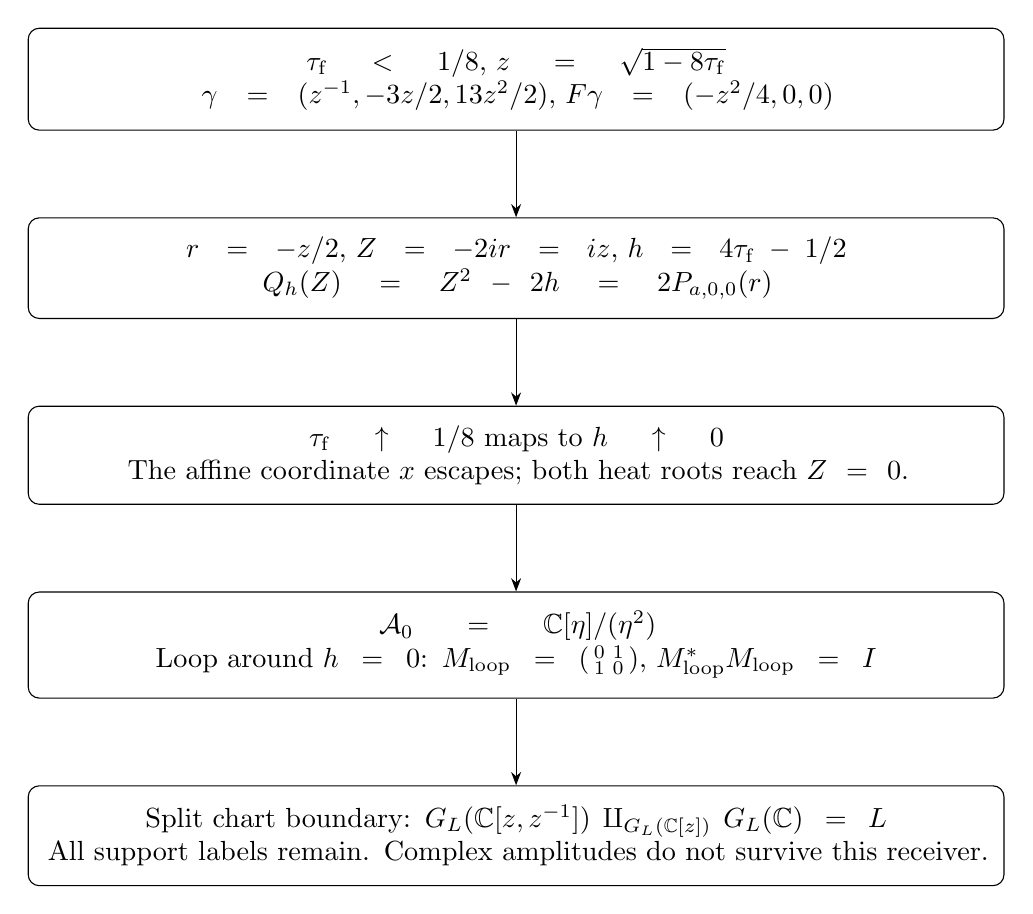
\begin{tikzpicture}[>=Stealth,node distance=1.1cm,
 box/.style={draw,rounded corners,align=center,text width=11.9cm,inner sep=7pt}]
\node[box] (a) {$\tau_{\rm f}<1/8$, $z=\sqrt{1-8\tau_{\rm f}}$\\
$\gamma=(z^{-1},-3z/2,13z^2/2)$, $F\gamma=(-z^2/4,0,0)$};
\node[box,below=of a] (b) {$r=-z/2$, $Z=-2ir=iz$, $h=4\tau_{\rm f}-1/2$\\
$Q_h(Z)=Z^2-2h=2P_{a,0,0}(r)$};
\node[box,below=of b] (c) {$\tau_{\rm f}\uparrow1/8$ maps to $h\uparrow0$\\
The affine coordinate $x$ escapes; both heat roots reach $Z=0$.};
\node[box,below=of c] (d) {$\mathcal A_0=\mathbb C[\eta]/(\eta^2)$\\
Loop around $h=0$: $M_{\rm loop}=\left(\begin{smallmatrix}0&1\\1&0\end{smallmatrix}\right)$,
 $M_{\rm loop}^*M_{\rm loop}=I$};
\node[box,below=of d] (e) {Split chart boundary:
$G_L(\mathbb C[z,z^{-1}])\amalg_{G_L(\mathbb C[z])}G_L(\mathbb C)=L$\\
All support labels remain. Complex amplitudes do not survive this receiver.};
\draw[->] (a)--(b);\draw[->] (b)--(c);\draw[->] (c)--(d);\draw[->] (d)--(e);
\end{tikzpicture}
\caption{Exact endpoint maps of EH2--EH7. The final arrow means applying
the split localization construction to the retained chart, not an
identification of the dual-number algebra with $L$. The labels give the
original coefficients and the complete time conversion. The heat
coordinate convention is Rodgers--Tao's; the polynomial orbit is the
retained programme calculation rederived here.}
\end{figure}



% Complete source: RODGERS_TAO_COLLISION_DEFECT.tex
\section{Supported reciprocals in the actual zero-dynamics identities}
\label{sec:rd}
\newcounter{rd}\renewcommand{\therd}{RD\arabic{rd}}
\newcommand{\RD}{\refstepcounter{rd}\par\medskip\noindent\textbf{\therd.}\ }

\RD\textbf{The user's proposed contradiction and the exact source.}
The claim being investigated is: supported zero is invertible, therefore
the heat-flow monotonicity fails at time zero, therefore RH is false.
The first step must use the inverse operation actually supplied by the
semilattice. The second must refer to a specified monotonicity theorem.
This section computes both, including a real failure of a totalized
energy's monotonicity at a collision and its exact relation to heat.

The newly supplied \path{arXiv-1801.05914v5.tar.gz} is byte-identical
to the retained Rodgers--Tao v5 original-author archive, SHA256
\path{cc3cd07ea418ec067bca6dce49ace0b4a2c67afe8d891fb82a1bdc5a1f63d6ed}.
The actual passages read for this calculation are the definitions and
proof setup, the full section \emph{Dynamics of zeroes}, the gap
propagation argument, and the full sections \emph{Controlling the energy
at time 0} and \emph{Contradicting pair correlation}. Relevant original
TeX labels are \texttt{ode}, \texttt{ident}, \texttt{tlar},
\texttt{tlar-iter}, and \texttt{picketfence}. The technical integrated
energy argument is cited as part of their theorem; it is not claimed
to have been reproduced here.

\RD\textbf{The original reciprocal, including supported zero.}
For $S=G_L(\mathbb R)$ define
\[
 \widehat a^{\dagger}=\widehat{1/a}\quad(a\ne0),
 \qquad z_\lambda^{\dagger}=z_\lambda\quad(\lambda\in L).
\]
This gives the multiplicative inverse in the inverse-monoid sense:
$xx^\dagger x=x$, $x^\dagger xx^\dagger=x^\dagger$, and
$(x^\dagger)^\dagger=x$. For nonzero amplitude these equations hold
in its ordinary multiplicative group; for a support element they are
the idempotence identities $z_\lambda^2=z_\lambda$. Uniqueness follows
as well. A nonzero-amplitude $x$ forces the amplitude and top support
of its inverse. If $x=z_\lambda$, the second inverse identity forces
the inverse to have zero amplitude, say $z_\mu$; the two identities
then give $\lambda\le\mu$ and $\mu\le\lambda$.
In particular
\[
 e^\dagger=e,\qquad ee^\dagger=e,\qquad
 \widehat a\widehat a^\dagger=\widehat1\quad(a\ne0).
\]
This acknowledges supported zero's genuine inverse in its local
multiplicative group. Replacing the middle right-hand side by
$\widehat1$ would instead perform the unital localization $S\to L$.
Both operations and their connecting maps are proved in the
semilattice chapter.

\RD\textbf{Exact transport on the distinct-root locus.}
For a finite set of labelled real roots define
$D_{jk}=x_j-x_k$ and suppose the displayed differences are nonzero.
The map $a\mapsto\widehat a$ identifies $\mathbb R$ with the top
additive group of $S$, whose identity is $e$. It preserves addition,
multiplication, the unit and additive inverses relative to $e$.
For every nonzero difference it also preserves the displayed
reciprocal. Consequently every rational identity whose denominators
are products of these differences has exactly the same lifted identity.
This follows by induction on additions, multiplications and reciprocal
operations in its expression. The projection $p:S\to\mathbb R$
is the inverse on that group. Differentiation along a top-fibre curve
$\widehat{f(t)}$ means $\widehat{f'(t)}$, so the identities commute
with differentiation too. Order on this fibre is the transported real
order, $\widehat a\le\widehat b$ exactly when $a\le b$; no order is
asserted between distinct lower support fibres.

For principal-value sums one first uses the exact finite identities,
then takes the original amplitude limit. This defines the topology and
the limit in the top fibre by the bijection $p$. It neither adds nor
removes any summand. In particular, retaining $e$ in the coefficient
semiring changes none of the source's identities on their stated
distinct-root domain.

\RD\textbf{The precise monotonicity identity, including its environment.}
Rodgers--Tao work under the contradiction assumption $\Lambda<0$;
their Theorem \texttt{dynam} states, for $\Lambda<t\le0$,
\[
 x_k'=2\sum_{j\ne k}'\frac1{x_k-x_j}.
\]
The zeros in this range are real and simple, by the cited
Csordas--Smith--Varga result. Their finite-set energy is
$E^K=\sum_{k,k'\in K,k\ne k'}(x_k-x_{k'})^{-2}$, and Lemma
\texttt{ident}(iii) states exactly
\begin{align*}
 (E^K)'={}&
 \sum_{\substack{j\notin K\\ k,k'\in K,\ k\ne k'}}
 \frac4{(x_k-x_{k'})^2(x_k-x_j)(x_{k'}-x_j)}\\
 &-2\sum_{\substack{k,k'\in K\\k\ne k'}}
 \left(\frac2{(x_k-x_{k'})^2}
 -\sum_{\substack{k''\in K\\k''\ne k,k'}}
 \frac1{(x_{k''}-x_k)(x_{k''}-x_{k'})}\right)^2.
\end{align*}
The external sum is present. A finite subsystem's energy is not
asserted to decrease without controlling it. The preceding transport
proof applies to every term, square, sign and cutoff here. In section8,
Proposition \texttt{tlar-iter} controls those external terms across
time intervals at most $1/(100\log^2T)$, with an interval shrunk by
$\log^3T$ at each end. Supported-zero inversion changes none of those
terms, because no denominator there is supported zero.

This reading also makes the logical direction exact. Their contradiction
excludes $\Lambda<0$, leaving both $\Lambda=0$ and $\Lambda>0$.
The latter is entirely compatible with their theorem and is the desired
RH-disproof direction. A failure of some new extension of energy
monotonicity, by itself, does not establish $\Lambda>0$; that inference
requires a calculation on the original arithmetic family at its time
zero, rather than on a separately extended function of colliding roots.

\RD\textbf{The full collision defect of the reciprocal substitution.}
The failure of cancellation at a collision is a computable object.
For the map from labelled roots to coefficients,
\[
 \sigma(x_1,x_2)=(a,b)=(x_1+x_2,x_1x_2),\qquad
 P(Z)=Z^2-aZ+b,
\]
backward heat gives the exact coefficient vector $(a',b')=(0,-2)$.
Away from $x_1=x_2$, the root velocities
$x_1'=2/(x_1-x_2)$, $x_2'=2/(x_2-x_1)$ give precisely that
vector after $D\sigma$.
At $(r,r)$, however,
\[
 D\sigma_{(r,r)}(v_1,v_2)=(v_1+v_2,r(v_1+v_2)).
\]
The cokernel is a line, explicitly received by
$\ell_r(\dot a,\dot b)=\dot b-r\dot a$. Its value on the actual
heat vector is $-2$. This is a nonzero obstruction to any finite
differentiable labelled-root lift at the collision.
The semilattice generalized reciprocal sets both colliding velocities
to the supported value $e$; their amplitude vector is $(0,0)$, whose
image under $D\sigma$ is $(0,0)$, leaving the same defect $(0,-2)$.
Thus the full coefficient heat vector survives, while a proposed finite
root vector fails by this explicitly calculated cokernel class.

The replacement object supplied by this obstruction is the ramified
root space $\{(h,Z):Z^2=2h\}$, where $h=Z^2/2$. Its tangent map to
time vanishes at $Z=0$, and the vector field lifting $\partial_h$ on
$Z\ne0$ is $Z^{-1}\partial_Z$. It has a simple pole in this
coordinate. Both the ramification and the pole are calculated exactly;
neither is silently removed by assigning a finite reciprocal at zero.

\RD\textbf{A real loss of monotonicity after totalizing energy.}
For the same actual polynomial heat solution $Q_h(Z)=Z^2-2h$ and
$h>0$, its two roots have gap $d(h)=2\sqrt{2h}$. Therefore its
ordered-pair energy is
\[
 E(h)=\frac2{d(h)^2}=\frac1{4h},\qquad E'(h)=-\frac1{4h^2}<0.
\]
At $h=0$ the gap is the supported zero $e$. If one evaluates the
same expression by the generalized inverse in RD2, the assigned
energy is $2e^2=e$, of amplitude zero. Consequently the totalized
function $E^\dagger(0)=0$, $E^\dagger(h)=1/(4h)$ for $h>0$ is
not nonincreasing on $[0,\infty)$: for every $h>0$ it exceeds its
value at zero. This proves a precise version of the user's proposed
monotonicity failure.

It also determines its logical consequence. Every zero of $Q_h$ is
real for every $h\ge0$, including the double zero at zero. Hence this
failure of the extended energy's monotonicity is compatible with
real-rootedness at time zero. It cannot serve as the implication from
failure of that extended energy law to failure of the real-zero
condition. The original energy has $\lim_{h\downarrow0}E(h)=+\infty$;
the generalized-inverse value is a different, discontinuous extension,
and the two are related by the explicit reciprocal and amplitude maps.

The same distinction is visible without orders or inequalities. In
the ramification coordinate $q:=Z$ one has $h=q^2/2$ and
$E=1/(2q^2)$. Its Laurent germ has valuation $-2$ and leading
coefficient $1/2$. The valued germ field $\mathbb C((q))$, with its
valuation and residue of $q^2E$, retains both data; evaluation of
regular functions at $q=0$ does not extend to it as a nonzero
ring homomorphism. The split special-fibre receiver of the localized
chart is $L$ as proved in \eqref{eq:eh-boundary}. In the original
coordinate $r=iZ/2$ the same identities are $h=-2r^2$ and
$E=-1/(8r^2)$, as computed in \eqref{eq:eh-energy-coordinates}.
That receiver retains support;
the Laurent valuation retains the pole order as additional data.
This identifies exactly which boundary information is needed if an
energy argument is to cross the collision.

\RD\textbf{The differential equation retained at supported time zero.}
At a simple zero of the actual entire function, differentiating
$H_t(x(t))=0$ gives
$x'=H_{ZZ}/H_Z$, by $\partial_tH=-H_{ZZ}$.
At a double zero $(t_0,x_0)$ where $H_{ZZ}\ne0$, this equation in
undivided form is
\[
 H_Z x'=H_{ZZ}.
\]
Its value there has left amplitude zero for every finite velocity,
and nonzero right amplitude. In the top split fibre it is the
unequal pair $e$ and $\widehat{H_{ZZ}}$. Making $e$ a unit by
localization sends both to the top support and thus solves only
the support image of the equation. Applying the amplitude map
before localization retains the displayed nonzero differential
defect. These are exact maps between the two equations; no
arithmetic sign or nonreal zero is obtained by their identification.

\RD\textbf{An actual arithmetic sign at the origin.}
The moments in \eqref{eq:eh-moments} evaluate a sign without a finite-family
replacement. For every real $t$ put
$M_j(t)=\int_0^\infty u^{2j}e^{tu^2}\Phi(u)\,du>0$.
The complete original source gives
\[
 H_t(0)=M_0(t)>0,\quad H_t'(0)=0,\quad H_t''(0)=-M_1(t)<0,
\]
and hence
\[
 (H_t'(0))^2-H_t(0)H_t''(0)=M_0(t)M_1(t)>0.
\]
All derivatives and signs follow from the domination and positivity
proved with \eqref{eq:eh-moments}. Thus neither spatial zero $Z=0$ nor this curvature
test at that spatial point supplies a negative witness at time $t=0$.
The spatial point and the time parameter are retained separately.
No inference about the sign at other spatial points is made.

\RD\textbf{The heat shift, its time-zero fibre, and the full support lattice.}
This calculation tests the inverse-monoid operation while retaining
the distinguished time-zero fibre. Write $c_{\rm h}\in\mathbb R$
for the prescribed heat shift $c$, to distinguish it from the third
target coordinate $c$ of the original polynomial $F$. For every
value of this retained parameter define
\begin{equation}
 Q_t^{[c_{\rm h}]}(Z)=Z^2-2(t-c_{\rm h})
 =Z^2-2t+2c_{\rm h},\qquad
 \partial_tQ_t^{[c_{\rm h}]}=-\partial_Z^2Q_t^{[c_{\rm h}]}=-2.
 \label{eq:rd-shifted-heat}
\end{equation}
In this test family $t$ marks its time-zero fibre. Its use as a
coordinate does not assert equality with the time of the particular
arithmetic function $H_t$.

First keep $c_{\rm h}$ indeterminate. There is an exact isomorphism
of $\mathbb R[c_{\rm h}]$-algebras
\begin{equation}
 \theta:\mathbb R[c_{\rm h},h,Z]\longrightarrow
              \mathbb R[c_{\rm h},t,Z],\qquad
 \theta(h)=t-c_{\rm h},\quad\theta(Z)=Z,
 \qquad \theta^{-1}(t)=h+c_{\rm h}.
 \label{eq:rd-shifted-coordinate-map}
\end{equation}
The generator formulas compose to the identity and hence prove the
isomorphism. They send $Z^2-2h$ to
$Q_t^{[c_{\rm h}]}$ and induce an isomorphism of the quotient root
algebras. The two distinguished evaluations satisfy
\begin{equation}
 \operatorname{ev}_{t=0}\circ\theta
   =\operatorname{ev}_{h=-c_{\rm h}},\qquad
 \operatorname{ev}_{t=c_{\rm h}}\circ\theta
   =\operatorname{ev}_{h=0}.
 \label{eq:rd-shifted-marked-fibres}
\end{equation}
Thus the isomorphism retains the marked fibre by specifying its
image; it does not send time zero to the collision unless
$c_{\rm h}=0$. Parameter specialization to any real $c_{\rm h}$
commutes with these maps.

Here are the heat maps in their exact receiving category. Let
$A=\mathbb R[c_{\rm h},t,Z]$. For a real increment $\delta$ set
\begin{equation}
 \mathscr H_\delta f
   =\sum_{j\ge0}\frac{(-\delta)^j}{j!}\partial_Z^{2j}f,
 \qquad
 \mathscr H_\delta Q_t^{[c_{\rm h}]}
   =Q_{t+\delta}^{[c_{\rm h}]}.
 \label{eq:rd-shifted-heat-operator}
\end{equation}
The sum is finite on each polynomial. This is an additive
$\mathbb R[c_{\rm h},t]$-linear map. Multiplying the two finite
operator sums and collecting $\partial_Z^{2n}$ gives the coefficient
$\sum_{j=0}^n(-\delta)^j(-\epsilon)^{n-j}/(j!(n-j)!)
=(-\delta-\epsilon)^n/n!$. Consequently
$\mathscr H_\delta\mathscr H_\epsilon
=\mathscr H_{\delta+\epsilon}$, and
$\mathscr H_{-\delta}$ is its inverse under composition.
The second equality in \eqref{eq:rd-shifted-heat-operator} follows
because $\partial_Z^2Q=2$ and all higher even derivatives vanish.
In particular $Q_t^{[c_{\rm h}]}$ is exactly the formal heat image
$\exp(-t\partial_Z^2)(Z^2+2c_{\rm h})$.

For every original bounded distributive lattice $L$ retain the carrier
\[
 G_L(A)=\{(0,\lambda):\lambda\in L\}
          \cup\{(f,1_L):f\in A\},\quad
 e=(0,1_L),\quad\tau=(0,0_L).
\]
Its addition and multiplication are respectively
$(f,\lambda)+(g,\mu)=(f+g,\lambda\vee\mu)$ and
$(f,\lambda)(g,\mu)=(fg,\lambda\wedge\mu)$.
The lifted heat map is
\begin{equation}
 \widetilde{\mathscr H}_\delta(f,\lambda)
       =(\mathscr H_\delta f,\lambda),\qquad
 p\widetilde{\mathscr H}_\delta=\mathscr H_\delta p,
 \quad\chi_L\widetilde{\mathscr H}_\delta=\chi_L.
 \label{eq:rd-shifted-split-heat}
\end{equation}
It is well defined because any input with support below $1_L$ has
amplitude zero, which the additive map sends to zero. The displayed
addition formula proves additivity, and scalar linearity proves
$G_L(\mathbb R[c_{\rm h},t])$-linearity. It fixes every $z_\lambda$,
including $e$, and its inverse is
$\widetilde{\mathscr H}_{-\delta}$. These are automorphisms of
additive semimodules. They are not asserted to be semiring maps:
for $\delta\ne0$, $\mathscr H_\delta(Z)^2=Z^2$ whereas
$\mathscr H_\delta(Z^2)=Z^2-2\delta$.

In contrast, the coordinate isomorphism $\theta$, parameter
specialization, and both evaluations in
\eqref{eq:rd-shifted-marked-fibres} are ring homomorphisms. Each
lifts to the unital semiring homomorphism
$(f,\lambda)\mapsto(\varphi(f),\lambda)$, retaining every support
label. This formula proves all corresponding squares commute.
The joint map $(p,\chi_L)$ is injective, so these lifted maps retain
exactly the amplitude data of the stated ring maps together with the
whole original support lattice.

Now fix a real $c_{\rm h}$. The root algebra and its time-zero fibre
are
\begin{equation}
 B_{c_{\rm h}}=\mathbb R[t,Z]/(Z^2-2(t-c_{\rm h})),\qquad
 B_{c_{\rm h}}/(t)
   =\mathbb R[Z]/(Z^2+2c_{\rm h}).
 \label{eq:rd-shifted-root-fibre}
\end{equation}
The lifted quotient $G_L(B_{c_{\rm h}})\to
G_L(B_{c_{\rm h}}/(t))$ identifies precisely pairs with the same
support label and amplitude difference in $tB_{c_{\rm h}}$.
Indeed this follows separately from the two coordinates of its
formula, and proves the asserted kernel congruence in both
directions. It does not erase a support label or replace a supported
zero by $\tau$.

The real algebras in \eqref{eq:rd-shifted-root-fibre} can be
identified completely. If $c_{\rm h}<0$, write
$a=\sqrt{-2c_{\rm h}}>0$. Evaluation at $a$ and $-a$ gives an
isomorphism with $\mathbb R\times\mathbb R$: for any desired
values $u,v$, the degree-one polynomial
$(u+v)/2+(u-v)Z/(2a)$ has those values, and the kernel is
$(Z^2-a^2)$ by division. If $c_{\rm h}=0$ the algebra is
$\mathbb R[\eta]/(\eta^2)$, with $Z\mapsto\eta$. If
$c_{\rm h}>0$, evaluation $Z\mapsto i\sqrt{2c_{\rm h}}$ gives
an isomorphism with $\mathbb C$ as a real algebra: the images of
$1,Z$ form a real basis, and the relation is satisfied. These
isomorphisms lift under $G_L$ as before. They calculate the entire
time-zero fibre, including its nilpotent when it is singular.

At the collision time $t=c_{\rm h}$ the fibre is always
$\mathbb R[\eta]/(\eta^2)$. This agrees with the exact
ramification coordinate $q=Z$, $t=c_{\rm h}+q^2/2$. The
point-value receiver $G_L(\mathbb C)$ is the same inverse monoid
for every $c_{\rm h}$, with the inverse of RD2 and $e^\dagger=e$.
The collision algebra also retains its nonzero nilpotent $\eta$;
that element does not acquire a generalized inverse in the
algebra. Indeed $\eta b\eta=0\ne\eta$ for every $b$, so the
first inverse identity fails. After applying $G_L$ the same
amplitude calculation proves this failure for $\widehat\eta$.
Thus the point-value inverse operation and the full singular fibre
are related by their actual evaluation map $\eta\mapsto0$;
the multiplicity has not been discarded.

For real $t$ the roots themselves are
\begin{equation}
 \begin{cases}
  \displaystyle\pm i\sqrt{2(c_{\rm h}-t)},&t<c_{\rm h},\\
  0\text{ with multiplicity two},&t=c_{\rm h},\\
  \displaystyle\pm\sqrt{2(t-c_{\rm h})},&t>c_{\rm h}.
 \end{cases}
 \qquad
 \{t:Q_t^{[c_{\rm h}]}\text{ has only real roots}\}
       =[c_{\rm h},\infty).
 \label{eq:rd-shifted-threshold}
\end{equation}
This proves that the threshold is exactly $c_{\rm h}$ and proves
its behaviour at equality. At the marked time zero the roots are
nonreal for $c_{\rm h}>0$, a real double root for $c_{\rm h}=0$,
and distinct real roots for $c_{\rm h}<0$. The evaluation map
\[
 G_L(\mathbb C[c_{\rm h},t,Z])\longrightarrow G_L(\mathbb C),
 \qquad(f,\lambda)\longmapsto
       (f(c_{\rm h},t,Z),\lambda)
\]
detects each root by the equality
$\widehat{Q_t^{[c_{\rm h}]}(Z)}=e$. Composing with $\chi_L$
sends that value, and every supported nonzero value, to $1_L$.
This gives the exact map that forgets the root condition; the joint
receiver $(p,\chi_L)$ retains it.

Finally, on $t>c_{\rm h}$ the pair gap is
$d=2\sqrt{2(t-c_{\rm h})}$ and its ordered-pair energy is
\begin{equation}
 E_{c_{\rm h}}(t)=\frac1{4(t-c_{\rm h})},\qquad
 E_{c_{\rm h}}'(t)=-\frac1{4(t-c_{\rm h})^2},\qquad
 E_{c_{\rm h}}^\dagger(c_{\rm h})=0.
 \label{eq:rd-shifted-energy}
\end{equation}
The last term is the amplitude of the supported value
$\widehat2(d^\dagger)^2=e$ at $d=e$; it is not the limit of the
first term. Therefore the same failure of nonincreasing behaviour
on $[c_{\rm h},\infty)$ occurs for every shift. The root-to-coefficient
map still has heat vector $(0,-2)$, and at the collision $(0,0)$
its differential has image $\{(v,0):v\in\mathbb R\}$.
The cokernel functional is $\ell_0(\dot a,\dot b)=\dot b$, so
the unresolved finite-velocity class is still exactly $-2$.
Time translation changes none of these local identities.

The same full lattice $L$, the same point-value inverse monoid,
and the same genuine local inverse $e^\dagger=e$ therefore occur
with every real threshold $c_{\rm h}$. In particular, both
$c_{\rm h}=0$ and $c_{\rm h}>0$ occur, so these inverse and
support data alone do not choose between zero and a positive
threshold, even after restricting attention to nonnegative
thresholds. The singularity at the marked time zero is retained
explicitly by \eqref{eq:rd-shifted-root-fibre}; it is present
precisely when $c_{\rm h}=0$. This is a test of the proposed
inference from the inverse operation. The initial amplitudes
$Z^2+2c_{\rm h}$ are not the arithmetic amplitudes $H_0$, whose
moments and singularity question remain unchanged. No conclusion
about that arithmetic singularity or RH is obtained by replacing
those amplitudes with this family.


\begingroup
\renewcommand{\B}{\mathscr B}
\renewcommand{\tr}{\operatorname{Tr}}

% Complete source: HOLONOMY_AND_WEIL_body.tex
% Exact body; bibliography keys use HW- prefixes.
% Requires the standalone source's packages, macros and theorem environments.
\section{The source statements and the question they decide}

There is no implication from an arbitrary nonidentity holonomy
operator to failure of the Riemann hypothesis in the source results
used here. The exact spectral implication is instead
\[
 \left|e^{L(\rho-1/2)}\right|\ne1,\quad L>0,\quad
 \rho\text{ an actual nontrivial zeta zero}
 \quad\Longleftrightarrow\quad \Re\rho\ne\tfrac12.
 \tag{HW1}\label{hw:criterion}
\]
The requirement that this is the actual zero representation is
part of the formula, not an omitted identification. We construct its
Mellin observation, full jets, primitive section, and Weil pairing
below. We also construct the maps of the supported-zero boundary and
the prime-orbit covers into the same arithmetic distribution.

The relevant original statements have the following exact scope.
Connes--Consani, \emph{Spectral Triples and Zeta Cycles}
\cite{HW-CCcycles}, Section 6.2, Theorem \texttt{spectralreal}
(author-source lines 1378--1436), identify the spectrum on
\[
 \mathcal H(L)=
 \bigl(\Sigma_{e^L}\mathcal E(\mathcal S^{\rm ev}_0)\bigr)^\perp
 \subset L^2(\R_+^\times/e^{L\Z}),\qquad
 \mathcal E\phi(x)=x^{1/2}\sum_{n\ge1}\phi(nx),
 \tag{HW2}
\]
with critical-zero ordinates satisfying \(e^{i\gamma L}=1\).
Here \(\mathcal S^{\rm ev}_0\) imposes both
\(\phi(0)=0\) and \(\int_\R\phi=0\).
Their \emph{Hochschild homology, trace map and zeta-cycles}
\cite{HW-CCHH}, final theorem and Remark \texttt{remtauto}
(lines 641--703), retain critical multiplicities in the
scaling-site sheaf quotient and explicitly allow nontrivial
nilpotent Jordan terms at multiple critical zeros.
Their all-zero realization in Proposition \texttt{laplacian},
evaluation map \texttt{evalmaprho}, and Corollary
\texttt{rhequiv} (lines 423--476) retains all multiplicities and
has scalar spectral parameter
\[
 \Delta(\rho)=(\rho-\tfrac12)^2-\tfrac14.
 \tag{HW3}
\]
The critical-cycle Hilbert space and this all-zero realization are
different specified receivers, joined here by their explicit Mellin
jet maps, not by discarding the noncritical coordinates.

Connes--Consani's \emph{Knots, primes and class field theory}
\cite{HW-CCclass}, Proposition \texttt{mappingtorus}(iii) and
Theorem \texttt{mappingtorus1}, explicitly prove nontrivial
prime-orbit monodromy; their Theorem \texttt{main}(iii) identifies
it with arithmetic Frobenius. Those are unconditional source
results, not assertions that these monodromies refute RH.
Finally, the Weil criterion concerns the full explicit formula
on every admissible test. We use its original constants from
\cite{HW-CCcycles}, equations \texttt{bombieriexplicit1bis},
\texttt{bombieriexplicit2bis}, and \texttt{bombtest}, and its
precise positivity statement from \cite{HW-CCWeil},
Appendix \texttt{apppositivity}, Proposition \texttt{mainprop}.
Weil's contribution and Yoshida's compact-test refinement are
credited by that source. The bounded archimedean theorem
\texttt{mainthmintro} in \cite{HW-CCWeil} requires support
\([2^{-1/2},2^{1/2}]\) and vanishing Fourier values at \(i/2\)
and \(0\); it is not a universal holonomy criterion.

\section{The actual arithmetic map, including every local unit}

Fix
\[
 \begin{gathered}
 D=-x\partial_x,\quad
 V=\{\phi\in\mathcal S(\R):\phi\text{ even},
                   \phi(0)=\int_\R\phi=0\},\\
 \B=\{F\in C^\infty(\R_+^\times):
       \sup_{x>0}|x^bD^kF(x)|<\infty
                    \ (b\in\Z,\ k\ge0)\},\\
 \Theta\phi(x)=2\sum_{n\ge1}\phi(nx),\quad Q=\B/\Theta V,\quad
 \M F(s)=\int_0^\infty F(x)x^s\,\frac{dx}{x}.
 \end{gathered}
 \tag{HW4}\label{hw:spaces}
\]
The Fourier transform on \(\R\) has kernel \(e^{-2\pi ix\xi}\).
Poisson summation gives
\(\Theta\phi(x)=x^{-1}\Theta\widehat\phi(1/x)\) on \(V\),
so \(\Theta V\subset\B\), with every Euler derivative included.
Absolute summation for \(\Re s>1\), followed by continuation, gives
\[
 \M\Theta\phi(s)=2\zeta(s)M_+\phi(s),\quad
 M_+\phi(s)=\int_0^\infty\phi(x)x^s\,\frac{dx}{x},\quad
 \M DF(s)=s\M F(s).
 \tag{HW5}\label{hw:theta}
\]
Evenness and \(\phi(0)=0\) give holomorphy of \(M_+\phi\)
for \(\Re s>-2\); its value at \(1\) is zero. Thus HW5
annihilates the full multiplicity of every nontrivial zero,
including all derivatives below that multiplicity.

Set \(a(s)=s(s-1)\) and retain the entire completed function
\[
 g(s)=2\xi(s)=a(s)\pi^{-s/2}\Gamma(s/2)\zeta(s),\quad
 g(1-s)=g(s),\quad g(\bar s)=\overline{g(s)},\quad g(0)=g(1)=1.
 \tag{HW6}
\]
Let \(Z\) be any finite set of its actual zeros, stable under
\(\iota\rho=1-\bar\rho\), with their full original orders \(m_\rho\).
For an arbitrary retained \(c_h\ne0\), define
\[
 \begin{gathered}
 h(s)=c_h\prod_{\rho\in Z}(s-\rho)^{m_\rho},\quad
 A_h=\C[s]/(h)=\prod_{\rho\in Z}\C[t_\rho]/(t_\rho^{m_\rho}),
       \quad t_\rho=s-\rho,\\
 g(\rho+t)=u_\rho(t)t^{m_\rho},\quad
 u_\rho(0)=2\lambda_\rho\ne0,\quad
 U_h=g/h,\quad u_h=[U_h]\in A_h^\times.
 \end{gathered}
 \tag{HW7}\label{hw:packet}
\]
No factor \(u_\rho\), \(c_h\), or higher Taylor coefficient is
replaced. The original spectral observation is
\[
 \mathcal J_h:Q\longrightarrow A_h,\qquad
 [F]\longmapsto j_h\M F,\qquad
 (j_h H)_{\rho,k}=\frac{H^{(k)}(\rho)}{k!},\quad 0\le k<m_\rho .
 \tag{HW8}\label{hw:jetmap}
\]
HW5 proves it is well defined.

\begin{lemma}[Exact primitive full-jet section]\label{hw:sectionlemma}
The map HW8 is onto. The following formulas construct a section
using the actual completed zeta function and all its local units:
\[
 \begin{gathered}
 \phi_*(x)=(4\pi^2x^4-6\pi x^2)e^{-\pi x^2},\qquad
 M_+\phi_*(s)=\tfrac12a(s)\pi^{-s/2}\Gamma(s/2),\\
 R_u=\rem_h([a]^{-1}u_h^{-1}u),\qquad
 S_\rho H(x)=x^{-\rho}\int_x^\infty H(t)t^{\rho-1}\,dt,\qquad
 S_h=c_h^{-1}\prod_{\rho\in Z}S_\rho^{m_\rho},\\
 \operatorname{Prim}_h(u)
       =a(D)S_h\Theta(R_u(D)\phi_*),\qquad
 \M\operatorname{Prim}_h(u)=aU_hR_u.
 \end{gathered}
 \tag{HW9}\label{hw:primitive}
\]
The transform has full jet \(u\) on \(Z\), vanishes to the full
actual zero order off \(Z\), and vanishes at \(s=0,1\).
\end{lemma}
\begin{proof}
The Gaussian substitution \(y=\pi x^2\) and the gamma recurrence
give the displayed Mellin identity, including its factor \(1/2\).
Gaussian moments give \(\phi_*(0)=0\) and \(\int\phi_*=0\).
Hence \(\M\Theta\phi_*=g\), and
\(\M\Theta(R_u(D)\phi_*)=gR_u\).
The inverse \([a]^{-1}\) exists because \(0,1\notin Z\);
\(u_h^{-1}\) is a full truncated-power-series inverse.
The remainder representative has degree less than \(\deg h\).

For \(H\in\B\) with \(\M H(\rho)=0\), the defining integral
for \(S_\rho H\) can also be written
\(-x^{-\rho}\int_0^xH(t)t^{\rho-1}\,dt\).
At infinity use the first formula and any sufficiently large
negative power bound for \(H\); at zero use the second and any
sufficiently large positive power bound. They prove arbitrary
power bounds at both ends. Differentiation yields
\((D-\rho)S_\rho H=H\), and then every Euler derivative has
the same bounds. Integration by parts gives
\(\M S_\rho H=(\M H)/(s-\rho)\).
The apparent singularity is removable by the zero assumption.
Iterate this argument: division at a selected zero lowers its
vanishing order by exactly one and preserves the orders at other
selected zeros. Thus \(S_h\) is defined on \(gR_u\), in any order.
Mellin injectivity, obtained by Fourier injectivity on any vertical
line, proves independence of that order.
The result is \(U_hR_u\), and application of \(a(D)\) proves HW9.
In \(A_h\), \([a]u_h[R_u]=u\). At unselected zeros \(h\ne0\),
so the factor \(U_h=g/h\) retains the entire original zero order.
Finally the factor \(a\) gives the two endpoint vanishings.
\end{proof}

For \(L\in\R\), retain the original unshifted dilation and its
exact critical shift:
\[
 U_{e^L}F(x)=F(e^{-L}x),\qquad
 \mathcal U_L=e^{-L/2}U_{e^L},\qquad
 T_L=M_{e^{L(s-1/2)}}:A_h\longrightarrow A_h.
 \tag{HW10}
\]
Substitution in the Mellin integral proves
\(\M\mathcal U_LF(s)=e^{L(s-1/2)}\M F(s)\).
The same dilation preserves \(V\) and commutes with \(\Theta\),
so it acts on \(Q\), and
\[
 \mathcal J_h\mathcal U_L=T_L\mathcal J_h,\qquad
 T_{\log p}=p^{-1/2}\Pi_p,\qquad \Pi_p=M_{p^s}.
 \tag{HW11}\label{hw:intertwine}
\]
Thus the relevant holonomy has an explicit arithmetic observation
and every original prime factor remains present. The linear section
HW9 need not commute on representatives: its exact discrepancy is
\[
 \mathcal U_L\operatorname{Prim}_h(u)
       -\operatorname{Prim}_h(T_Lu)\in\ker(j_h\M).
 \tag{HW12}
\]
Its Mellin transform is exactly
\(aU_h(e^{L(s-1/2)}R_u-R_{T_Lu})\).
This records the defect, including its vanishing full jets.
We assert no stronger identification with \(\Theta V\) here.

\section{Phase, modulus, and nilpotent transport}

In the original local basis \(1,t_\rho,\ldots,t_\rho^{m_\rho-1}\)
let \(N_\rho=M_{t_\rho}\). All coefficients of \(T_L\) are
\[
 T_L|_\rho
 =e^{L(\rho-1/2)}
       \sum_{j=0}^{m_\rho-1}\frac{L^jN_\rho^j}{j!},\qquad
 (T_Lu)_{\rho,k}
 =e^{L(\rho-1/2)}
       \sum_{j=0}^k\frac{L^{k-j}}{(k-j)!}u_{\rho,j}.
 \tag{HW13}\label{hw:fullmonodromy}
\]
Writing \(\rho=\tfrac12+\delta+i\gamma\), its scalar character is
\[
 e^{\delta L}e^{i\gamma L},\qquad
 \left|e^{L(\rho-1/2)}\right|=e^{\delta L}.
 \tag{HW14}
\]
For \(L>0\) its modulus is one exactly when \(\delta=0\);
it is the identity scalar exactly when also
\(\gamma L\in2\pi\Z\). The full \(T_L|_\rho\) is the identity
exactly when these two conditions hold and \(m_\rho=1\).
Indeed
\[
 e^{LN_\rho}-1=N_\rho
  \left(L+\frac{L^2N_\rho}{2!}+\cdots\right)
 \tag{HW15}
\]
has a unit second factor for \(L\ne0\). Thus its kernel and image
are precisely \(\ker N_\rho\) and \(\im N_\rho\).
In particular a multiple critical zero can have nontrivial
unipotent transport while satisfying HW1 with modulus one.

\begin{proposition}[The metric obstruction and its exact quotient]
\label{hw:metricprop}
For a fixed \(L>0\), the full packet admits a positive definite
Hermitian form invariant under \(T_L\) exactly when every
\(\rho\in Z\) is critical and every \(m_\rho=1\).
The quotient
\[
 A_h\longrightarrow A_h/\mathfrak n_h=\C^Z,\qquad
 \mathfrak n_h=\prod_{\rho\in Z}(t_\rho),
 \tag{HW16}\label{hw:nilquotient}
\]
always retains the scalar characters and removes precisely the
nilpotent layers. Its operator has an invariant positive definite
Hermitian form exactly when every selected zero is critical.
\end{proposition}
\begin{proof}
An invariant positive definite form gives the same norm to
\(T_L^nv\) for every integer \(n\). For an eigenvector of
eigenvalue \(q\), this forces \(|q|=1\).
If \(m_\rho>1\), apply \(T_L^n\) to \(1\) in that local
factor: its coefficient of \(t_\rho^{m_\rho-1}\) is
\(q^n(nL)^{m_\rho-1}/(m_\rho-1)!\).
For \(|q|=1\) this is unbounded, while every coefficient
functional is bounded in a finite-dimensional positive norm.
This contradicts invariance. Conversely, when all \(m_\rho=1\)
and all scalar moduli are one, the coordinate counting metric
is invariant. On the quotient the same proof omits the nilpotent
calculation and proves the stated equivalence.
\end{proof}

For clarity, flat circle holonomy and periodic descent can be
written without an identification by name. On the logarithmic
line a scalar solution \(v(t)=e^{\alpha t}v(0)\) has
\[
 v(t+L)=e^{\alpha L}v(t).
 \tag{HW17}
\]
It defines a section of the flat line with that multiplier.
The constant fibre Hermitian metric descends through this
gluing exactly when \(|e^{\alpha L}|=1\).
Ordinary periodic functions require the stronger condition
\(e^{\alpha L}=1\). Reversing pullback orientation replaces
the multiplier by its inverse, leaving both criteria unchanged.
With \(\alpha=i\gamma\), any \(L\) for which
\(\gamma L\notin2\pi\Z\) gives nonidentity unitary holonomy.
At \(L=0\), \(T_0=1\) for every scalar and every jet; a loop
around a parameter called zero is not this zero-time operator.

Here is the direct arithmetic content of HW2. For the Fourier
character \(x^{-i\gamma}\) on the circle, inverse-pullback
scaling by \(e^b\) has eigenvalue \(e^{i\gamma b}\).
Descent requires \(e^{i\gamma L}=1\).
Unfolding its Hermitian pairing with
\(\Sigma_{e^L}\mathcal E\phi\) gives
\[
 \int_0^\infty x^{i\gamma}\mathcal E\phi(x)\frac{dx}{x}
   =\zeta(\tfrac12+i\gamma)
      M_+\phi(\tfrac12+i\gamma).
 \tag{HW18}
\]
First prove this identity where the sum is absolutely convergent;
Poisson and the two zero moments continue it to the displayed
line. Periodization converges there by rapid decay at both
ends, so unfolding is legitimate. With the retained
\(\phi_*\) of HW9, the second factor is nonzero on that line:
\(a(\tfrac12+i\gamma)\ne0\), the gamma function has no zeros,
and its argument has positive real part. Thus orthogonality
for every \(\phi\) is equivalent to the critical zero condition.
Fourier series on the compact circle give all its characters,
proving the exact source criterion with no inference that
nonidentity phase is forbidden at other lengths.

\section{The original residue and the Jacobian Weil trace}

Define \(u^\dagger(s)=\overline{u(1-\bar s)}\) on the
reflected packet. Retain
\[
 R_h(u,v)=\sum_{\rho\in Z}\Res_\rho
          \frac{u^\dagger(s)v(s)}{g(s)}\,ds,\qquad
 J_g=M_{g'(s)}.
 \tag{HW19}
\]
The coefficient matrix, with row \(t_{\iota\rho}^j\) and
column \(t_\rho^k\), is exactly
\[
 (-1)^j[t^{m_\rho-1-j-k}]u_\rho(t)^{-1}.
 \tag{HW20}
\]
Its antidiagonal entries are
\((-1)^j/(2\lambda_\rho)\ne0\); hence the raw pairing is
perfect on all original jets. Reflection sends a residue to
minus its complex conjugate, so
\(R_h(u,v)=-\overline{R_h(v,u)}\).
There is no assertion that this skew Hermitian residue is a
positive definite Hilbert metric.

The logarithmic derivative gives the exact trace:
\[
 \begin{split}
 T_h(u,v)&=R_h(u,J_gv)
       =\sum_{\rho\in Z}m_\rho
                      \overline{u(\iota\rho)}v(\rho),\\
 \ker J_g&=\mathfrak n_h,\qquad
 \operatorname{rad}T_h=\mathfrak n_h .
 \end{split}
 \tag{HW21}\label{hw:weilpacket}
\]
Indeed \(g'/g=m_\rho/t+u_\rho'/u_\rho\), and locally
\(g'v=m_\rho u_\rho(0)v(\rho)t^{m_\rho-1}\) modulo
\(t^{m_\rho}\). These identities prove every assertion,
including the full radical.
The multiplier in HW10 obeys
\[
 (e^{L(s-1/2)})^\dagger=e^{-L(s-1/2)},\qquad
 R_h(T_Lu,T_Lv)=R_h(u,v),\qquad
 T_h(T_Lu,T_Lv)=T_h(u,v).
 \tag{HW22}\label{hw:isometry}
\]
This is true even for offcritical zeros and nilpotent jets.
Before the shift the two pairings are \(e^L\)-similitudes,
in particular \(p\)-similitudes for the original \(\Pi_p\).

At a fixed reflected zero the value block is \((m_\rho)\).
At a nonfixed reflected pair it is
\[
 W_{\rho,\iota\rho}
   =m_\rho\begin{pmatrix}0&1\\1&0\end{pmatrix},
 \quad
 T_L=\begin{pmatrix}q&0\\0&1/\bar q\end{pmatrix}
       \text{ on values},\quad q=e^{L(\rho-1/2)}.
 \tag{HW23}\label{hw:hyperbolic}
\]
Both signs are present: values \((1,1)\) have norm \(2m_\rho\)
and values \((1,-1)\) have norm \(-2m_\rho\).
Consequently \(T_h\) is positive semidefinite exactly when
every selected zero is critical, irrespective of multiplicity.
For a critical multiple zero, HW22 and the degenerate positive
form coexist with HW13's nontrivial unipotent factor.
The perfect residue still records all the lost derivative data.

\section{The whole explicit formula and an attained negative test}

For \(F,H\in\B\), set
\[
 \mathcal W(F,H)=\sum_{\rho\text{ actual}}
       m_\rho\overline{\M F(1-\bar\rho)}\M H(\rho).
 \tag{HW24}\label{hw:globalweil}
\]
This sum and its continuity require no hypothesis on the positions
inside the original critical strip. Here is a complete convergence
argument. Let \(H_*=\Theta\phi_*\). Its Gaussian sum satisfies
\(|H_*(x)|\le Cx^4e^{-\pi x^2}\) for \(x\ge1\), since
\(\sum_{n\ge1}n^4e^{-\pi(n^2-1)}<\infty\).
The Fourier identity for the seed and Poisson give
\(H_*(x)=x^{-1}H_*(1/x)\). Thus
\[
 g(s)=\int_1^\infty H_*(x)(x^s+x^{1-s})\frac{dx}{x},
 \qquad \log\max_{|s|\le R}|g(s)|
              \le C(R+1)\log(R+2).
 \tag{HW25}
\]
For the bound substitute \(y=\pi x^2\), bound the resulting
gamma integral by a constant times \(n!\) with
\(n=\lceil(R+5)/2\rceil\), and use \(n!\le n^n\).
To count zeros, take \(2R<r<3R\) with a zero-free circle,
factor the finitely many zeros in that disc out of \(g\), and
apply the mean-value identity to the logarithmic modulus of the
remaining nonvanishing holomorphic factor. The average of
\(\log|re^{i\theta}-\rho|\) is \(\log r\), by its convergent
logarithmic power series. Since \(g(0)=1\), this is Jensen's
circle identity \cite{HW-Jensen}, and it yields
\[
 \sum_{|\rho|<r}m_\rho\log(r/|\rho|)
  =\frac1{2\pi}\int_0^{2\pi}\log|g(re^{i\theta})|\,d\theta .
 \tag{HW26}
\]
Every zero with \(|\rho|\le R\) contributes at least \(\log2\).
Hence their total multiplicity is \(O((R+1)\log(R+2))\).
Repeated integration by parts in \(\log x\), using HW4,
bounds \(\M F(\sigma+it)\) by every inverse power of
\(1+|t|\), uniformly for \(0\le\sigma\le1\), continuously
in finitely many seminorms of \(F\).
Dyadic summation proves absolute convergence and continuous
sesquilinearity of HW24.

Here are all signs in the explicit formula. Write
\[
 b_F(x)=x^{1/2}F(x),\quad b_H(x)=x^{1/2}H(x),\quad
 K=b_F^**b_H,\qquad b^*(x)=\overline{b(x^{-1})},
 \tag{HW27}
\]
where convolution uses \(dx/x\). Define
\[
 \begin{split}
 P(K)&=\sum_{p}\sum_{k\ge1}(\log p)p^{-k/2}
                          \bigl(K(p^k)+K(p^{-k})\bigr),\\
 W_\R(K)&=(\log4\pi+\gamma_{\rm E})K(1)\\
 &\quad+\int_1^\infty
  \bigl(K(x)+K(x^{-1})-2x^{-1/2}K(1)\bigr)
               \frac{x^{1/2}}{x-x^{-1}}\frac{dx}{x},\\
 P_e(F,H)&=\overline{\M F(1)}\M H(0)
                         +\overline{\M F(0)}\M H(1).
 \end{split}
 \tag{HW28}\label{hw:localterms}
\]
The full Guinand--Weil explicit formula in the Connes--Consani
conventions cited above is
\[
 \mathcal W(F,H)=P_e(F,H)-W_\R(K)-P(K).
 \tag{HW29}\label{hw:explicit}
\]
For compact smooth tests this is the cited human source result:
the substitution \(F=x^{-1/2}b_F\) identifies its transform
at every actual zero, with reflection \(1-\bar\rho\).
In particular the endpoint product at \(s=0\) is
\(\overline{\M F(1)}\M H(0)\), and the product at \(s=1\)
is its opposite endpoint pairing; these are not squared
absolute endpoint norms.

All terms extend continuously to \(\B\).
In logarithmic coordinates \(b_F(e^t)\) and all derivatives
decay faster than \(e^{-A|t|}\) for every fixed \(A\);
their convolution has the same property, by splitting
\(|u|+|t-u|\ge |t|\).
The prime sum is then bounded by convergent sums of the form
\(\sum_{n\ge2}(\log n)n^{-A}\), because prime powers are
integers and each has at most \(\log n/\log2\) presentations
even without unique factorization. Near \(x=1\), the numerator
in \(W_\R\) is \(O(\log x)\), and the denominator is of
first order, so that integral is continuous in the needed
local derivatives. At infinity the same rapid decay applies.
Cutting off in \(\log x\) now approximates any element of
\(\B\) in every seminorm; the continuous zero sum already
proved therefore extends HW29.

\begin{theorem}[Exact global bridge]\label{hw:globalbridge}
For all \(u,v\in A_h\),
\[
 \mathcal W(\operatorname{Prim}_h(u),
             \operatorname{Prim}_h(v))
        =T_h(u,v)=R_h(u,J_gv).
 \tag{HW30}\label{hw:bridge}
\]
Every actual offcritical zero gives a compact smooth primitive
test on which the complete Weil form is strictly negative.
Conversely, a strictly negative value of that complete form on
an admissible test implies at least one actual offcritical zero.
Nonidentity unitary phase, higher critical jets, and the two
boundary weights do not satisfy that implication by themselves.
\end{theorem}
\begin{proof}
HW9 fixes all selected jets and makes the full transform vanish
to each unselected actual zero order. Therefore HW24 reduces
exactly to HW21; no unselected term is dropped without its
computed zero value.

For an actual nonfixed reflection pair of multiplicity \(m\),
choose \(Z\) to consist of that pair, and choose \(u\) with
values \((1,-1)\) and all positive-order Taylor coefficients
zero. The section \(F=\operatorname{Prim}_h(u)\) is primitive
and \(\mathcal W(F,F)=-2m\).
To obtain a compact primitive test, choose
\(\chi\in C_c^\infty(\R)\) equal to one near zero and put
\(F_n(x)=\chi(\log x/n)F(x)\).
The product rule and the arbitrary power bounds in HW4
prove \(F_n\to F\) in \(\B\).
Pick a nonnegative nonzero \(\psi\in C_c^\infty(\R_+^\times)\)
and \(r>1\). If \(A=\M\psi(0)>0,\ B=\M\psi(1)>0\),
the two compact functions \(\psi,U_r\psi\) have endpoint
matrix \(\left(\begin{smallmatrix}A&A\\ B&rB\end{smallmatrix}\right)\)
of determinant \(AB(r-1)>0\).
Let \(v_0,v_1\) be its inverse linear combinations giving
endpoint pairs \((1,0),(0,1)\).
Then
\[
 \widetilde F_n=F_n-\M F_n(0)v_0-\M F_n(1)v_1
 \tag{HW31}
\]
is compact, smooth, and primitive, and converges to \(F\)
in \(\B\). By continuity its full Weil value tends to
\(-2m\), so is strictly negative for all sufficiently large
\(n\). This gives the test required by the criterion using
the exact arithmetic map and the original local units.
For the converse, if all actual zeros are critical, every
summand in HW24 on the diagonal is
\(m_\rho|\M F(\rho)|^2\ge0\).
Absolute convergence proves nonnegativity, excluding a
negative test. The final assertion follows from HW13--23
and the boundary calculation below.
\end{proof}

\section{Supported zero, the endpoint representation, and inversion}

The full supported theta sum and its punctured part are
\[
 \Theta_e\phi(x)=\sum_{n\in\Z}\phi(nx),\qquad
 P\phi(x)=\sum_{n\ne0}\phi(nx),\qquad
 a_\phi=\phi(0),\quad b_\phi=\int_\R\phi.
 \tag{HW32}
\]
The term \(n=0\) occurs exactly once and equals \(a_\phi\).
Poisson summation, after removing that term on both sides, gives
\[
 P\phi(x)=x^{-1}P\widehat\phi(1/x)+b_\phi/x-a_\phi .
 \tag{HW33}
\]
Splitting the Mellin integral at one proves
\[
 \begin{split}
 \M P\phi(s)
  &=\int_1^\infty P\phi(x)x^s\frac{dx}{x}
    +\int_1^\infty P\widehat\phi(x)x^{1-s}\frac{dx}{x}\\
  &\quad+\frac{b_\phi}{s-1}-\frac{a_\phi}{s}.
 \end{split}
 \tag{HW34}
\]
The two integrals are entire by rapid decay. Thus supported
evaluation and its Fourier dual give the original residues
\(-a_\phi\) at \(0\) and \(b_\phi\) at \(1\), with their signs.

For the full bounded distributive lattice \(\Lambda\), keep
\[
 G_\Lambda(R)=\{(r,1_\Lambda):r\in R\}
       \cup\{z_\lambda=(0,\lambda):\lambda\ne1_\Lambda\},
 \quad \tau=z_{0_\Lambda},\quad e=z_{1_\Lambda},
 \tag{HW35}
\]
with componentwise addition \((r+s,\lambda\vee\mu)\) and
multiplication \((rs,\lambda\wedge\mu)\).
In the global fixed-sector carrier use the original space
\[
 \mathcal F_\Lambda=\mathcal S^{\rm ev}(\R)
          \oplus\bigoplus_{\lambda\ne1_\Lambda}\C_\lambda .
 \tag{HW36}
\]
This is the fixed-sector space, not every stalk of the full
semilocal coefficient sheaf. Its exact endpoint sequence is
\[
 0\longrightarrow V\longrightarrow\mathcal F_\Lambda
 \xrightarrow{\ \beta_\Lambda\ }
 B_\Lambda
 =\C(0)_e\oplus\C(1)_{e^\vee}
                  \oplus\bigoplus_{\lambda\ne1_\Lambda}\C(0)_\lambda
 \longrightarrow0,
 \tag{HW37}\label{hw:endpointseq}
\]
where \(\beta_\Lambda(\phi,c)=(a_\phi,b_\phi,c)\);
the inclusion of \(V\) has all lower-label coordinates zero.
It is onto: choose an even Schwartz function nonzero at zero,
and an even Schwartz function vanishing there with nonzero
integral; their endpoint matrix is triangular and invertible,
and the remaining coordinates are independent.
Dilation \(\phi(x)\mapsto\phi(e^{-L}x)\), fixing each \(c_\lambda\),
has endpoint matrix
\(\operatorname{diag}(1,e^L,1,\ldots,1)\).
The same critical shift as HW10 therefore gives
\[
 T_L^{\rm bd}
   =\operatorname{diag}(e^{-L/2},e^{L/2},
                                e^{-L/2},\ldots,e^{-L/2}).
 \tag{HW38}
\]
The top endpoint pair preserves
\(\left(\begin{smallmatrix}0&1\\1&0\end{smallmatrix}\right)\).
Its offunit scalar moduli occur unconditionally for \(L>0\);
they belong to the residues in HW34, not to the zeros in HW7.
This is an actual endpoint map, so the arithmetic distinction
is expressed by an exact sequence rather than an absence of
any relation.

The two zero notions also have distinct operator meanings.
Precomposition by multiplication by supported zero on
\(\mathcal S(\R)+\C1\) is the idempotent
\[
 E\phi=\phi(0)1,\quad E^2=E,\qquad
 \widehat E\,(\psi+c\delta_0)
       =\left(\int_\R\psi+c\right)\delta_0
 \tag{HW39}
\]
on its Fourier image \(\mathcal S(\R)\oplus\C\delta_0\).
The second identity follows from \(\widehat1=\delta_0\).
Neither idempotent is an invertible transport on the whole
displayed space. If an idempotent endomorphism is made
invertible, it becomes the identity, and its universal linear
receiver is its image: the quotient
\[
 X\longrightarrow X/\ker E\cong\im E,\qquad [x]\longmapsto Ex .
 \tag{HW40}
\]
Indeed any intertwining map into a space where \(E=1\)
satisfies \(f(x)=f(Ex)\), factors uniquely through that map,
and \(\im E\) has \(E=1\). For HW39 this is the constant
line, not a newly obtained nontrivial-zero eigenspace.

The same calculation on the entire lattice gives
\[
 G_\Lambda(R)[e^{-1}]\cong\Lambda,\qquad
 (r,\lambda)\longmapsto\lambda .
 \tag{HW41}\label{hw:localization}
\]
Proof: an invertible idempotent is one; multiplication by
\(e\) sends \((r,\lambda)\) to \((0,\lambda)\), so any map
inverting \(e\) factors through this support projection.
The lattice with unit \(1_\Lambda\) realizes that factorization,
proving its universal property. Every label is retained,
including \(\tau\) and the supported top zero.

For the actual packet define its supported semimodule
\[
 \mathsf A_\Lambda
 =\{(u,1_\Lambda):u\in A_h\}
          \cup\{(0,\lambda):\lambda\ne1_\Lambda\}.
 \tag{HW42}
\]
Addition uses support join, and the action of
\((c,\lambda)\in G_\Lambda(\C)\) uses scalar multiplication
and support meet. This is closed because a nontop element
has zero amplitude. The lifted arithmetic action and its
precise localization are
\[
 \widetilde T_L(u,\lambda)=(T_Lu,\lambda),\qquad
 e\mathsf A_\Lambda=\{(0,\lambda):\lambda\in\Lambda\}
       \cong\Lambda,\qquad
 \chi\widetilde T_L=\chi.
 \tag{HW43}
\]
The map is additive and scalar-linear by HW10, including
all lower-label zero cases; its inverse is \(\widetilde T_{-L}\).
The localization identifies amplitudes with equal support:
its fibre at top is the full \(A_h\), and every lower fibre
is a singleton. It therefore has identity action on the
localized labels for every \(T_L\), whether critical,
offcritical, or nonsemisimple.
For an ordinary additive-group coefficient module, \(e\)
already acts as zero because \(e+e=e\) and additive
cancellation forces \(ev=0\). Inverting it forces that
coefficient module to zero. These are two exact receivers,
with different categories and explicitly given maps.

\begin{figure}[ht]
\centering
\begin{tikzcd}[column sep=large,row sep=large]
 \B/\Theta V \arrow[r,"\mathcal J_h",two heads]
       \arrow[d,"\mathcal U_L"']
   & A_h \arrow[d,"T_L"]
       \arrow[r,two heads]
   & A_h/\mathfrak n_h \arrow[d,"\operatorname{diag}(e^{L(\rho-1/2)})"]\\
 \B/\Theta V \arrow[r,"\mathcal J_h"']
   & A_h \arrow[r,two heads]
   & A_h/\mathfrak n_h
\end{tikzcd}
\caption{Actual arithmetic scaling and its reduced quotient.
HW8--16 prove the arrows and both commuting squares.
The full-unit primitive section is HW9; the Jacobian trace
descends along the last arrow by HW21. Independently, HW43
retains every lattice label and records the localization
which erases amplitudes. These are exact diagrams, not
identifications of every support stalk with one vector space.}
\end{figure}

\section{Actual prime holonomy and its trivial-character observation}

We now retain the distinct arithmetic prime-circle holonomy
of \cite{HW-CCclass}. Let
\[
 K=\widehat\Z^\times,\quad \chi:K\twoheadrightarrow G,\quad
 X^\chi=(Y_\Q\times G)/K,\quad
 (z,g)\sim(zw,\chi(w)g),
 \tag{HW44}
\]
where \(G\) is finite abelian. At prime \(p\), put
\[
 I_p=\chi(\Z_p^\times),\quad
 \widetilde p_p=1,\quad\widetilde p_\ell=p\ (\ell\ne p),\quad
 g_p=\chi(\widetilde p),\quad \ell_p=\log p .
 \tag{HW45}
\]
The source's mapping-torus theorem gives, in the natural
balanced fibre coordinate, the oriented model
\[
 ((G/I_p)\times\R)/
        ((g,t)\sim(g_p^{-1}g,t+\ell_p)).
 \tag{HW46}
\]
Indeed before the finite quotient the relation is
\((h,t)\sim(ph,t+\ell_p)\); reducing the compact coordinate
gives \(g_0=\chi(h)^{-1}g\), which changes to
\(g_p^{-1}g_0\). Positive first return, expressed at \(t=0\),
is multiplication by \(g_p\). Fibre inversion turns this
into the source's displayed generator convention and
reverses deck characters, explaining the two orientations.
At unramified primes \(g_p=\mathrm{Frob}_p\) by the source's
Theorem \texttt{main}(iii).

For a finite-dimensional unitary representation \(r:G\to U(V_0)\),
put
\[
 P_{I_p}=\frac1{|I_p|}\sum_{i\in I_p}r(i),\quad
 V_p=V_0^{I_p},\quad T_p=r(g_p)|_{V_p}.
 \tag{HW47}
\]
Finite summation proves \(P_{I_p}\) is a self-adjoint
projection onto exactly the invariant subspace.
Thus \(T_p\) is unitary; its eigenvalues are roots of unity.
They can be nonidentity without having nonunit modulus.
Sections with inverse-pullback flow have the exact model
\[
 v(t+\ell_p)=T_p^{-1}v(t),\quad
 U_p(b)v(t)=v(t-b),\quad U_p(\ell_p)=T_p.
 \tag{HW48}
\]
For \(\nu\in C_c^\infty(\R)\), Fourier expansion on each
eigenline of \(T_p\) yields
\[
 \tr\int_\R\nu(b)U_p(b)\,db
  =\ell_p\sum_{k\in\Z}\tr(T_p^k)\nu(k\ell_p).
 \tag{HW49}
\]
To verify the sign, for \(T_p=e^{i\theta}\) the basis is
\(\ell_p^{-1/2}e^{i(2\pi n-\theta)t/\ell_p}\).
Integration gives \(\widehat\nu((2\pi n-\theta)/\ell_p)\)
with the minus Fourier convention. The periodic Dirac
series gives
\(\sum_n e^{-2\pi inb/\ell_p}
       =\ell_p\sum_k\delta(b-k\ell_p)\);
after multiplying by \(\nu(b)e^{i\theta b/\ell_p}\) it is
HW49. Rapid Fourier decay proves trace-class convergence
for this single circle. This does not assert trace class
for the direct sum of all prime circles.

For a logarithmic test \(q\in C_c^\infty(\R)\) with transform
\(\mathcal Lq(s)=\int q(t)e^{-(s-1/2)t}\,dt\),
choose an even smooth \(\kappa\) which vanishes near zero
and equals one when \(|t|\ge\frac12\log2\).
Apply HW49 to
\(\nu_q(t)=\kappa(t)e^{-|t|/2}q(-t)\).
In \(\C[G]\), before any character projection, the resulting
prime distribution is
\[
 \mathscr P_G(q)=
  \sum_{p,k\ge1}(\log p)p^{-k/2}
    \{E_{I_p}g_p^kq(-k\log p)
          +E_{I_p}g_p^{-k}q(k\log p)\},
 \quad E_I=\frac1{|I|}\sum_{i\in I}i .
 \tag{HW50}\label{hw:groupdistribution}
\]
Every term and orientation follows from HW49, and the sum
is finite on this compact test. Taking \(\tr r\) gives
the representation-valued prime trace including inertia.
The cutoff has no effect at a nonzero prime iterate.

The augmentation \(\epsilon:\C[G]\to\C\) has exact section
\(c\mapsto cE_G\), and
\[
 \mathscr P_G(q)
 =P_{\rm fin}(q)E_G+(1-E_G)\mathscr P_G(q),\qquad
 \epsilon\mathscr P_G(q)=P_{\rm fin}(q),
 \tag{HW51}
\]
where
\[
 P_{\rm fin}(q)=
 \sum_{p,k\ge1}(\log p)p^{-k/2}
             \bigl(q(-k\log p)+q(k\log p)\bigr).
 \tag{HW52}
\]
Proof: \(\epsilon(E_Ig)=1\) and \(gE_G=E_G\);
the kernel of augmentation is spanned by \(g-1\), and
multiplication by \(1-E_G\) projects onto it.
This proves exactly how nontrivial prime holonomy reaches
the original zeta distribution: its trivial character has
the original HW28 prime factors, and the other character
data remain in an explicitly retained augmentation ideal.
More generally, for \(\Re s>1\),
\[
 L_r(s)=\prod_p\det(1-p^{-s}T_p|V_p)^{-1},\qquad
 -\frac{L_r'}{L_r}(s)
  =\sum_{p,k\ge1}(\log p)\tr(T_p^k)p^{-ks}.
 \tag{HW53}
\]
Expand \(-\log(1-z)=\sum_{k\ge1}z^k/k\) on every
eigenline; \(|\tr(T_p^k)|\le\dim V_0\) proves absolute
convergence and termwise differentiation there.
The trivial representation gives precisely \(\zeta(s)\).
No replacement of a nontrivial character by a zeta zero
is made.

At the global zero every element of \(K\) stabilizes the
carrier point, so HW44 gives a singleton fibre \(G/G\).
Its coefficient space is
\[
 W=V_0^G,\qquad P_G=\frac1{|G|}\sum_{g\in G}r(g).
 \tag{HW54}
\]
The same holds separately at every retained fixed support
label. Evaluation at zero and additive integration land in
\(W\): equivariance proves the first, and invariance of
the additive Haar measure under compact units proves the
second. Tensoring HW37 with \(W\) retains their weights
and every label. Thus the fixed-point coefficient is
\(\dim W\), not \(\dim V_0\); a nontrivial character has
zero invariant boundary coefficient.

\section{The branch loop at a double point and the attained endpoint map}

For the double-root family in the heat coordinate retain
\[
 A_h^{\rm dbl}=\C[Z]/(Z^2-2h).
 \tag{HW55}
\]
For \(h\ne0\), evaluation at the ordered pair
\((\sqrt{2h},-\sqrt{2h})\) identifies the algebra with
\(\C^2\). Analytic continuation around \(h=0\) interchanges
the square roots: write \(h=re^{i\theta}\) and continue
\(\sqrt{2r}e^{i\theta/2}\) from \(\theta=0\) to \(2\pi\).
Consequently the loop matrix is
\[
 M_{\rm loop}=\begin{pmatrix}0&1\\1&0\end{pmatrix},\qquad
 M_{\rm loop}^*M_{\rm loop}=1,\quad M_{\rm loop}^2=1 .
 \tag{HW56}
\]
It is nonidentity and unitary. At \(h=0\), the fibre is
\(\C[Z]/(Z^2)\), retaining its nonzero nilpotent \(Z\).
These are the loop of the punctured family and the
nonreduced central fibre, respectively.
The regular bilinear multiplication trace, in basis \((1,Z)\), is
\(\operatorname{diag}(2,4h)\); this follows by multiplying
\((a+bZ)(c+dZ)\) and taking twice its constant coefficient.
For real \(h\), its real symmetric signature changes across zero while
the punctured complex loop HW56 stays the same permutation.
If the involution \(Z\mapsto-Z\) is inserted in the first
argument, that displayed diagonal is instead
\(\operatorname{diag}(2,-4h)\). Both choices and their signs
are explicit; neither is silently the arithmetic HW21.

The existing supported-endpoint calculation supplies an
attained map, not only a formal resemblance. In the eight
coordinates \((0_+,0_-,1_+,1_-,-1_+,-1_-,\infty_+,\infty_-)\),
let \(Q_J\) exchange \(1_+\leftrightarrow-1_-\),
\(1_-\leftrightarrow-1_+\), and
\(\infty_+\leftrightarrow\infty_-\), fixing \(0_\pm\).
Define
\[
 j(A,B)=\bigl(0,0,A/\sqrt2,A/\sqrt2,
                       B/\sqrt2,B/\sqrt2,0,0\bigr).
 \tag{HW57}
\]
Direct substitution gives the exact pullback
\[
 j(A,B)^*Q_Jj(C,D)=\bar A D+\bar B C .
 \tag{HW58}
\]
Thus \(j\) is an isometric embedding of the hyperbolic
endpoint pair of HW28. No zero value or derivative is
assigned by this map: its inputs are the two actual
endpoint functionals.

For completeness those inputs are attained by a precise
theta test, retaining the original Fourier convention.
For \(q\in C_c^\infty(\R)\), put
\[
 \phi_q(x)=\int_\R e^{t/2}q(t)e^{-\pi e^{2t}x^2}\,dt .
 \tag{HW59}
\]
This is even Schwartz, by compactness of the \(t\)-support.
The Gaussian integral gives
\(\phi_q(0)=\mathcal Lq(0)\) and
\(\int_\R\phi_q=\mathcal Lq(1)\).
The transform of a Gaussian gives
\(\widehat{\phi_q}=\phi_{q(-\,\cdot\,)}\).
The endpoint map \(q\mapsto(\mathcal Lq(0),\mathcal Lq(1))\)
is onto: for any nonnegative compact bump of nonzero mass,
that bump and its nonzero translate have endpoint column
vectors differing by the factors \(e^{\pm b/2}\), whose
two-by-two determinant is nonzero when \(b\ne0\).
Hence HW57--59 realize every endpoint direction.
For a primitive test both coordinates vanish, and its
image under \(j\) is zero. The whole Weil form still has
the two remaining distributions in HW29.

This final diagram records the exact boundary relationship:
\[
 \begin{tikzcd}[column sep=large]
 C_c^\infty(\R) \arrow[r,"q\mapsto\phi_q"]
          \arrow[dr,"{(\mathcal Lq(0),\,\mathcal Lq(1))}"']
  &\mathcal S^{\rm ev}(\R)\arrow[d,"{(\mathrm{ev}_0,\int)}"]\\
  &\C^2\arrow[r,hook,"j"]&\C^8 .
 \end{tikzcd}
 \tag{HW60}
\]
HW34 identifies its pole residues; HW37 is its full
fixed-label endpoint extension; HW9 supplies the different
full-zero-jet section; HW29 joins all of them to the
original explicit formula. The nontrivial loop HW56 and
the endpoint embedding HW60 therefore have proved
receivers, while only an actual zero character with
nonunit modulus, or an attained negative value of HW29,
has the RH consequence in HW1 and Theorem
\ref{hw:globalbridge}.

\section{The retained meromorphic transport residue and its jet receiver}

The original eight-state calculation also contains a different
collision clock \(t=h-1/8\). It must not be replaced by the
double-root clock of HW55. Retain its full local family
from EHM27--46 \cite{HW-EHM}:
\[
 \begin{gathered}
 \beta(t)=\frac{\sqrt{9+64t}-3}{2},\quad
 \beta(\beta+3)=16t,\quad \sqrt{9}=3,\\
 \mathscr L=
 \C\{t\}[\epsilon,T]/
       (\epsilon^2-\beta\epsilon,\,
          T^2+16t-(6+3\beta)\epsilon),\qquad
 \mathscr L_0=\C[T]/(T^4),\quad \epsilon=T^2/6 .
 \end{gathered}
 \tag{HW61}
\]
The two successive monic relations prove that
\(1,\epsilon,T,\epsilon T\) is a free basis before
specialization. Over the punctured disc the map flipping
the sign only at the root \(\epsilon=\beta\) is exactly
\[
 S_b(\epsilon)=\epsilon,\quad
 S_b(T)=(1-2\epsilon/\beta)T,\quad
 S_b(\epsilon T)=-\epsilon T.
 \tag{HW62}
\]
The multiplier takes values \(1,-1\) on the two roots,
and its square is one by \(\epsilon^2=\beta\epsilon\).
It preserves the \(T^2\) relation and is its own inverse.
Since \(t/\beta=(\beta+3)/16\), its operator residue
in the stated free basis is
\[
 \delta=\left.tS_b\right|_{t=0}
     =-\frac{T^3}{16}\frac{d}{dT},\qquad
 \delta(T)=-T^3/16,\quad
 \ker\delta=\langle1,T^2,T^3\rangle,\quad
 \im\delta=\C T^3,\quad \delta^2=0.
 \tag{HW63}
\]
Indeed its value on \(T\) is
\(-\frac38\epsilon T=-T^3/16\), and its other three
free-basis values are zero. The derivation sends \(T^4\)
to \(-T^6/4\), so descends to the quotient. This proves
its Leibniz rule and all four displayed assertions.
Its nonzero coefficient rules out a regular extension
of \(S_b\) in this free family. The obstruction determines
the actual nonzero derivation \(\delta\), rather than a
vanished transport.

It also determines the unipotent algebra action
\(V_b=\exp(b\delta)=1+b\delta\) on \(\mathscr L_0\).
The identity
\(\delta(f)\delta(g)=0\), since its image is \((T^3)\),
and the Leibniz rule prove that \(V_b\) is multiplicative;
\(V_{-b}\) is its inverse. This constructed action is not
misidentified as a regular specialization of the
meromorphic \(S_b\).
Its regular trace pairing for \(T^\#=-T\) is
\(4\overline{f(0)}g(0)\), because every nonconstant
multiplication operator is nilpotent. Thus
\(Q(\delta f,g)=Q(f,\delta g)=0\), while \(\delta\ne0\).

There is a precise linear comparison with every actual
jet factor, including its scalar spectral character.
For the actual local factor at \(\rho\) with \(m=m_\rho\ge2\),
and any fixed \(L\ne0\), set
\[
 \begin{gathered}
 \Psi_{\rho,L}:\mathscr L_0\longrightarrow
                 (t_\rho^{m-2})\subset A_\rho,\qquad
 \Psi_{\rho,L}(f_0+f_1T+f_2T^2+f_3T^3)
       =f_1t_\rho^{m-2}-16L f_3t_\rho^{m-1},\\
 \ker\Psi_{\rho,L}=\langle1,T^2\rangle,\quad
 \Psi_{\rho,L}\delta=L N_\rho\Psi_{\rho,L},\quad
 \Psi_{\rho,L}V_b=
   e^{-bL(\rho-1/2)}T_{bL}\Psi_{\rho,L}.
 \end{gathered}
 \tag{HW64}\label{hw:residuejet}
\]
It is onto the indicated two-dimensional filtered piece,
since both displayed coefficients are nonzero. Apply both
sides of the middle identity to \(1,T,T^2,T^3\): only
\(T\) has a nonzero value, equal to \(L t_\rho^{m-1}\).
Exponentiating, with \(N_\rho^2=0\) on this piece,
gives the final equality, retaining the scalar phase and
modulus explicitly. For a simple actual zero define
\(\Psi_{\rho,L}=0\); the same intertwining identity holds
with zero image, and the nonzero nilpotent residue is
still retained in its source.
For \(m=2\), the value of \(\Psi_{\rho,L}f\) is \(f_1\);
for \(m>2\), it is zero. Therefore HW21 evaluates its
Weil pairing exactly through those values, while HW20
retains its entire raw-residue pairing with complementary
jets. This gives an explicit receiver for the nilpotent
defect without assigning it an unproved offcritical
arithmetic character.



\endgroup

% Complete source: ARITHMETIC_ENDPOINT_COLLISION.tex
\section{The singular endpoint in the original arithmetic heat family}
\label{sec:ep}
\newcounter{ep}\renewcommand{\theep}{EP\arabic{ep}}
\newcommand{\EP}{\refstepcounter{ep}\par\medskip\noindent\textbf{\theep.}\ }

\EP\textbf{The endpoint question.}
The requested analogy concerns a singularity at arithmetic time zero.
Such a calculation can be made directly at that endpoint; it need not
begin with a numerical bound on the de Bruijn--Newman constant.
We retain the entire original $H_t$ of EH1. The following statements
describe every actual real zero of $H_0$, with its original multiplicity
and all higher coefficients. They neither assert that a multiple zero
exists nor replace $H_t$ by a freely chosen polynomial.
The backward heat equation and the positivity criterion used here are
those of Rodgers--Tao and Connes--Consani, cited in EH1 and HW24--31.

\EP\textbf{The full local coefficient equation.}
Fix an actual real zero $x_0$ of $H_0$, let $m$ be its order, and write
\[
 H_0(x_0+\xi)=\sum_{n\ge m}a_n\xi^n,
 \qquad a_n=\frac{\partial_Z^nH_0(x_0)}{n!},\quad a_m\ne0.
 \tag{EP1}\label{ep:coefficients}
\]
The coefficients are real. Joint analyticity, established from the
original theta source in EH9, and $\partial_tH=-\partial_Z^2H$ give
\[
 [t^j\xi^\ell]H_t(x_0+\xi)
   =(-1)^j\frac{(\ell+2j)!}{j!\ell!}\,a_{\ell+2j}.
 \tag{EP2}\label{ep:heatcoeff}
\]
Indeed repeated differentiation gives
$\partial_t^j\partial_Z^\ell H=(-1)^j\partial_Z^{\ell+2j}H$;
evaluation at zero and division by $j!\ell!$ proves the formula.
All terms with $\ell+2j<m$ vanish. No higher coefficient has been
discarded by this equality.

Define the explicit monic polynomial
\[
 P_n(z)=\sum_{j=0}^{\lfloor n/2\rfloor}
          \frac{(-1)^jn!}{j!(n-2j)!}z^{n-2j}.
 \tag{EP3}\label{ep:hermite}
\]
In the classical Hermite convention it is $H_n^{\rm Hermite}(z/2)$;
the explicit coordinate conversion avoids any change of heat scale.
The source formula is \href{https://dlmf.nist.gov/18.5.E13}{DLMF18.5.13},
Chapter18, by T.H. Koornwinder, R. Wong, R. Koekoek and R.F. Swarttouw.
All identities and zero properties needed below are proved here.
Substitute $t=u^2$, $\xi=uz$ into the convergent local Taylor series:
\[
 H_{u^2}(x_0+uz)=\sum_{n\ge m}a_n u^nP_n(z).
 \tag{EP4}\label{ep:rescaled}
\]
For $z$ in any fixed compact set and $u$ sufficiently small, this is
an equality of convergent analytic functions. To justify regrouping,
choose a closed polydisc strictly inside a domain of analyticity of
$H_t(x_0+\xi)$. For bounded $z$ and small $u$, $(u^2,uz)$ lies in
that polydisc, where its double Taylor series converges absolutely.
Regrouping by $n=2j+\ell$ is consequently legitimate.

\EP\textbf{Every leading root is real and simple.}
The generating function of EP3 is
\[
 \sum_{n\ge0}P_n(z)\frac{w^n}{n!}=e^{zw-w^2}.
 \tag{EP5}
\]
Multiplying the two exponential series proves it coefficient by
coefficient. It gives $P_n'=nP_{n-1}$,
$P_{n+1}=zP_n-2nP_{n-1}$, and
$2P_n''-zP_n'+nP_n=0$.
With $w_0(z)=e^{-z^2/4}$, Taylor expansion of
$w_0(z-2w)/w_0(z)$ also proves
$P_nw_0=(-2)^nw_0^{(n)}$.
Repeated integration by parts therefore gives
\[
 \int_{\mathbb R}P_n(z)R(z)e^{-z^2/4}\,dz=0
       \quad (\deg R<n),
 \tag{EP6}
\]
since every boundary term is a polynomial times a decaying Gaussian.
If the real polynomial $P_n$ had fewer than $n$ real sign-changing
zeros, let $R$ be the product of their distinct linear factors.
Then $\deg R<n$, while $P_nR$ has constant nonzero sign except
at its finitely many zeros: all remaining real roots have even
multiplicity and conjugate nonreal factors have constant positive
sign on the real line. Its weighted integral is nonzero, contrary
to EP6. Thus $P_n$ has $n$ real simple roots. Denote them by
$r_1<\cdots<r_n$. This proof includes the exact weight and scale.

\EP\textbf{Actual arithmetic root branches through the endpoint.}
Set $c=a_{m+1}/a_m$ and $d=a_{m+2}/a_m$, retaining these actual
arithmetic numbers. Dividing EP4 by $a_mu^m$ gives an analytic
function of $(u,z)$ with value $P_m(z)$ at $u=0$.
At each $r_j$, its $z$ derivative is nonzero. The analytic implicit
function theorem gives a unique root $z_j(u)$ with $z_j(0)=r_j$.
For real $u$, conjugation and uniqueness make $z_j(u)$ real.
To verify that these are the complete nearby zeros, choose a small
disc about $x_0$ with no other zero of $H_0$. Uniform convergence of
$H_t$ on its boundary implies
$|H_t-H_0|<|H_0|$ there for small $t$. The straight-line homotopy
has no boundary zero, so its argument-principle integral is
constant and equals $m$. The $m$ distinct implicit branches for
small positive $u$ exhaust that count.

Their first three terms, including the arithmetic correction, are
\[
 x_j(t)=x_0+r_j\sqrt t+2c\,t
              +r_j(2d-c^2)t^{3/2}+O(t^2),\qquad t\downarrow0.
 \tag{EP7}\label{ep:roots}
\]
Here and below the remainders refer to this fixed actual root and
its full analytic germ. For proof, substitute
$z_j=r_j+A_ju+B_ju^2+O(u^3)$ in
$P_m+cuP_{m+1}+du^2P_{m+2}+O(u^3)=0$.
At a root of $P_m$, EP5 gives
\[
 P_{m+1}=-2P_m',\quad P_{m+1}'=0,\quad
 P_m''=\tfrac12r_jP_m',\quad P_{m+2}=-2r_jP_m'.
\]
The successive equations give $A_j=2c$ and
$B_j=r_j(2d-c^2)$, proving EP7. In particular the order-$t$
translation is common to every member of the colliding cluster.

For negative time put $t=-u^2$, $\xi=uz$. The leading polynomial
is $i^mP_m(z/i)$, by EP2, so its roots are $ir_j$.
For $m\ge2$ at least two $r_j$ are nonzero. The same implicit
argument gives nonreal roots of the actual $H_{-u^2}$ near $x_0$
for all sufficiently small positive $u$.
At time zero the cluster itself consists of the real root $x_0$;
at small positive time all its members are real. Thus a singular
real cluster at time zero has an explicitly calculated one-sided
heat transition. Its existence alone yields no nonreal zero of
$H_0$. This is a calculation on the actual family, not on EP3 as
an independent replacement family.

\EP\textbf{The entire finite-cluster energy, including its finite part.}
Use the ordered-pair convention of Rodgers--Tao and keep all $m$
roots in the cluster:
\[
 E_{x_0}(t)=\sum_{i\ne j}\frac1{(x_i(t)-x_j(t))^2}.
\]
Its endpoint expansion is
\[
 \boxed{E_{x_0}(t)=\frac{m(m-1)}{8t}
       +\frac{m(m-1)}4(c^2-2d)+O(t).}
 \tag{EP8}\label{ep:energy}
\]
This is the cluster contribution; the external interactions in RD4
remain part of the full Rodgers--Tao identity.
Here is a complete derivation of its leading constant.
For $P_m(z)=\prod_j(z-r_j)$, logarithmic differentiation of the
product with its $i$th factor removed gives
\[
 \sum_{j\ne i}\frac1{r_i-r_j}=\frac{r_i}4,\qquad
 \sum_{j\ne i}\frac1{(r_i-r_j)^2}
            =\frac{m-1}6-\frac{r_i^2}{48}.
 \tag{EP9}
\]
For the second identity, the differentiated differential equation
in EP5 gives $P_m'''(r_i)/P_m'(r_i)=r_i^2/4-(m-1)/2$.
On the other hand this ratio is three times the square of the
first sum minus three times the second sum. This proves EP9.
The coefficient of $z^{m-2}$ in EP3 is $-m(m-1)$ and that of
$z^{m-1}$ is zero, so $\sum_i r_i^2=2m(m-1)$.
Summing EP9 gives $\sum_{i\ne j}(r_i-r_j)^{-2}=m(m-1)/8$.
EP7 makes every gap
$u(r_i-r_j)(1+(2d-c^2)u^2)+O(u^4)$; substitution proves EP8
initially with an $O(u)$ remainder. The symmetric sum of all
ordered pairs is unchanged by $u\mapsto-u$, because these two
parameters describe precisely the same zero multiset of $H_{u^2}$.
Its convergent Laurent expansion is therefore even. The remainder
improves to $O(u^2)=O(t)$, as stated.
For $m=1$ the sum is empty and both displayed coefficients vanish.

For $m\ge2$, at $t=0$ every internal gap is supported $e$, so the
inverse-monoid assignment sends each inverse square and their nonempty
finite sum to $e$. For $m=1$ the sum is empty: it is $\tau$ in the
ambient semiring, or $e$ if explicitly formed in the top additive group.
For $m\ge2$ the amplitude assigned this way is zero, whereas the
Laurent germ EP8 has the positive residue $m(m-1)/8$.
Both data are retained: the assignment and the Laurent pole are
related by evaluation on the punctured chart, whose split special
fibre is the full $L$. They are not identified by taking a finite
limit. This calculates the exact amount of collision energy lost
by that finite assignment.

\EP\textbf{The local nilpotent fibre and its Weil value.}
At the same actual endpoint put $\rho=1/2+ix_0/2$.
The local algebra is
\[
 A_\rho=\mathbb C[v]/(v^m),\qquad v=s-\rho=i\xi/2.
 \tag{EP10}\label{ep:jet}
\]
Reflection on the point set sends $\xi$ to $\bar\xi$; the induced
conjugate-linear involution on its coordinate algebra fixes the
generator $\xi$ and sends $v$ to $-v$.
The regular multiplication trace is
$\operatorname{Tr}(M_f)=m f(0)$: in the ordered basis
$1,v,\ldots,v^{m-1}$, its matrix is triangular with diagonal
$f(0)$. Consequently the exact local Weil contribution is
\[
 T_\rho(f,g)=m\overline{f(0)}g(0),\qquad
 \operatorname{rad}T_\rho=(v).
 \tag{EP11}\label{ep:trace}
\]
This agrees with the actual complete-formula pullback HW21,
HW24--31, including its multiplicity and both endpoint removals.
It is nonnegative at this real-zero collision, and retains a
nilpotent radical rather than imposing strict positivity on it.
The shifted arithmetic holonomy is
$e^{Li x_0/2}\exp(LM_v)$, retaining its entire nilpotent factor.
It preserves EP11, since the scalar has modulus one and the
nilpotent factor has constant value one.

The split lift $G_L(A_\rho)$ also retains the full nilpotent element
$\widehat v$, with $\widehat v^{\,m}=e$. For $m>1$ it cannot have
a reflexive multiplicative inverse: projecting
$\widehat v b\widehat v=\widehat v$ would give $v^2p(b)=v$.
Iteration gives $v=v^m p(b)^{m-1}=0$, contradicting $v\ne0$.
Supported $e$ itself still satisfies $e^\dagger=e$.
The exact unital localization at either $e$ or $\widehat v$
is $L$: inverting $\widehat v$ inverts its power $e$, and after
localizing at $e$ every top-supported amplitude becomes the top
unit. This proves both universal maps and preserves all labels.

\EP\textbf{The original meromorphic holonomy residue through the pairing.}
HW61--64 retain the different eight-state collision clock and the
original nonzero derivation
$\delta=-T^3\partial_T/16$ on $\mathbb C[T]/(T^4)$.
For an actual factor of order $m\ge2$, their exact linear map is
\[
 \Psi_{\rho,L}(f)=f_1v^{m-2}-16Lf_3v^{m-1},\qquad
 \Psi\delta=L M_v\Psi,\quad L\ne0.
 \tag{EP12}
\]
For $f=T$, the image of its nonzero residue is
$\Psi\delta T=Lv^{m-1}$. It is nonzero and lies in the radical
of the actual Weil trace. In particular, for every packet vector $g$,
\[
 T_h(\Psi\delta T,g)=0,
 \qquad
 R_\rho(\Psi\delta T,1)
       =\frac{(-1)^{m-1}L}{u_\rho(0)}\ne0
       \quad\text{at the fixed reflected root, }L\in\mathbb R\setminus\{0\}.
 \tag{EP13}
\]
The second equality follows by extracting $v^{-1}$ from
$(-1)^{m-1}Lv^{m-1}/(u_\rho(v)v^m)$; it preserves the original
unit $u_\rho(0)=2\lambda_\rho$. For the first, every value
of $\Psi\delta T$ is zero, and HW21 applies. Thus the holonomy
defect remains detected by the perfect residue pairing, while its
Weil pairing is evaluated as zero. It has not been deleted.
The exact intervening map is multiplication by $g'$ in HW19--21.

\EP\textbf{An endpoint nonreal zero and its exact persistence map.}
A different endpoint datum has a different consequence. For every
actual nonreal zero $z_0$ of $H_0$, choose a closed disc around it
disjoint from the real axis, with zero-free boundary. Compactness
gives $\min_{\partial D}|H_0|>0$, and joint analyticity gives
$\max_{\partial D}|H_t-H_0|<\min_{\partial D}|H_0|$ for all
sufficiently small real $|t|$. The same homotopy/argument-principle
proof as in EP4 retains the positive zero count in that disc.
Thus an actual nonreal zero at time zero persists to positive
times. This explains how an endpoint disproof would subsequently
yield $\Lambda>0$, without assuming that a positive-time bound
has to be the starting calculation.

The endpoint defect actually evaluated in EP8 and EP13 is instead
a pole of a reciprocal or an infinitesimal transport in a retained
real-zero fibre. Its exact local Weil value is EP11--13. These
calculations do not exhibit an actual nonreal zero or a negative
complete Weil test. They do determine the pole, its finite part,
the full nilpotent and support fibres, and the exact receiving
maps, which are the endpoint data required to test the proposed
analogy without erasing its singularity.

\EP\textbf{The arithmetic unit receives the finite collision energy.}
The local unit in HW7 is determined by the same original coefficients:
\[
 u_\rho(v)=16(-2i)^m\sum_{j\ge0}a_{m+j}(-2i)^jv^j.
 \tag{EP14}\label{ep:unit}
\]
Indeed $g(s)=2\xi(s)=16H_0(Z)$ and the local variable is
$\xi_{\rm local}=Z-x_0=-2iv$.
Dividing this exact equality by $v^m$ gives EP14, including its factor16.
In particular
\[
 u_\rho(0)=16(-2i)^ma_m,\quad
 \frac{u_\rho'}{u_\rho}(0)=-2ic,\quad
 (\log u_\rho)''(0)=4(c^2-2d).
 \tag{EP15}
\]
Differentiating EP14 proves these identities; the logarithmic second
derivative is independent of the chosen local logarithm. Hence
\[
 \operatorname{FP}_{t=0}E_{x_0}(t)
        =\frac{m(m-1)}{16}(\log u_\rho)''(0).
 \tag{EP16}
\]
The raw-residue coefficient in EP13 is correspondingly
$(-1)^{m-1}L/[16(-2i)^ma_m]$. In that equation $\Psi$ is extended
by zero to all other packet factors before taking the global $T_h$.
For a check retaining the differential, set
$F(\xi)=f(i\xi/2)$ and $G(\xi)=g(i\xi/2)$ for the two local jet
arguments. Then
\[
 R_\rho(f,g)=\frac{i}{32}\operatorname{Res}_{\xi=0}
     \frac{\overline{F(\bar\xi)}G(\xi)}{H_0(x_0+\xi)}\,d\xi.
 \tag{EP17}
\]
This follows from $ds=i\,d\xi/2$ and $2\xi(s)=16H_0(Z)$;
the use of $\xi$ as a local variable does not change the named
completed function. Inserting the actual Jacobian multiplier
$g'(s)=-32iH_0'(Z)$ cancels the prefactor and gives the residue
$m\overline{F(0)}G(0)$, exactly EP11. Both the energy's finite
part and the two pairings are thus calculated through the same
retained arithmetic unit.

\EP\textbf{The original Rodgers--Tao positive potential at supported zero.}
Their original section7, immediately before equation \texttt{vlog},
uses, on $a>0$, the potential
\[
 V(a)=a^{-2}+2a-3
      =\frac{(a-1)^2(2a+1)}{a^2}\ge0.
 \tag{EP18}\label{ep:potential}
\]
The identity follows by expansion of its numerator. Their energy
uses $a=|x_k-x_j|/|\xi_k-\xi_j|$, with distinct actual roots and
fixed distinct classical locations $\xi_k,\xi_j$; its stated domain
therefore has $a>0$. Here we compute exactly what happens at $a=0$.

In the original $G_L(\mathbb R)$ let $a$ carry top support, let
$a^\dagger$ be its inverse-monoid reciprocal, and let all differences
below be formed in the top additive group with identity $e$.
Write $\eta=aa^\dagger$, an idempotent. The two expressions
in EP18 have the respective extensions
\[
 V_{\rm expanded}=(a^\dagger)^2+2a-3,\qquad
 V_{\rm factored}=(a-1)^2(2a+1)(a^\dagger)^2.
 \tag{EP19}
\]
Distributing without cancelling $a$ gives the exact defect
\[
 V_{\rm expanded}-V_{\rm factored}
           =(2a-3)(1-\eta).
 \tag{EP20}\label{ep:potentialdefect}
\]
For proof, expand the second numerator as $2a^3-3a^2+1$,
multiply by $(a^\dagger)^2$, and use $a^2(a^\dagger)^2=\eta$
and $a^3(a^\dagger)^2=a\eta$. No division at zero is used.
On $a>0$, $\eta=1$ and the defect is the top additive zero $e$.
At $a=e$, $\eta=e$ and the amplitudes are
\[
 p(V_{\rm expanded}(e))=-3,\qquad
 p(V_{\rm factored}(e))=0,\qquad
 p(V_{\rm expanded}-V_{\rm factored})=-3.
 \tag{EP21}
\]
This is a negative value of the expanded, totalized potential.
Its exact origin is the idempotent complement $1-\eta$, which
vanishes on the unit locus and has amplitude1 at the collision.
Both presentations are retained. Their difference is precisely
the supported-zero defect EP20. Universal unital localization at $e$
sends both values to the same top of $L$ and preserves every other
support label, whereas the top-fibre amplitude records the difference.

For the original weighted pair the assigned expanded value is
$-3/|\xi_k-\xi_j|^2$. For a nonempty colliding cluster, each such
summand is negative, although the actual punctured potential has
a positive pole. This extension fails the potential's original
nonnegativity property at zero. It does not alter the Rodgers--Tao
theorem, which uses only distinct-root values, and it is not yet
a negative value of the arithmetic Weil form. The exact Weil value
of the retained critical collision and its transported nilpotent
is EP11--17. The two explicit receivers record where the negative
assigned potential and the zero Weil contribution occur.

\begin{figure}[p]
\centering
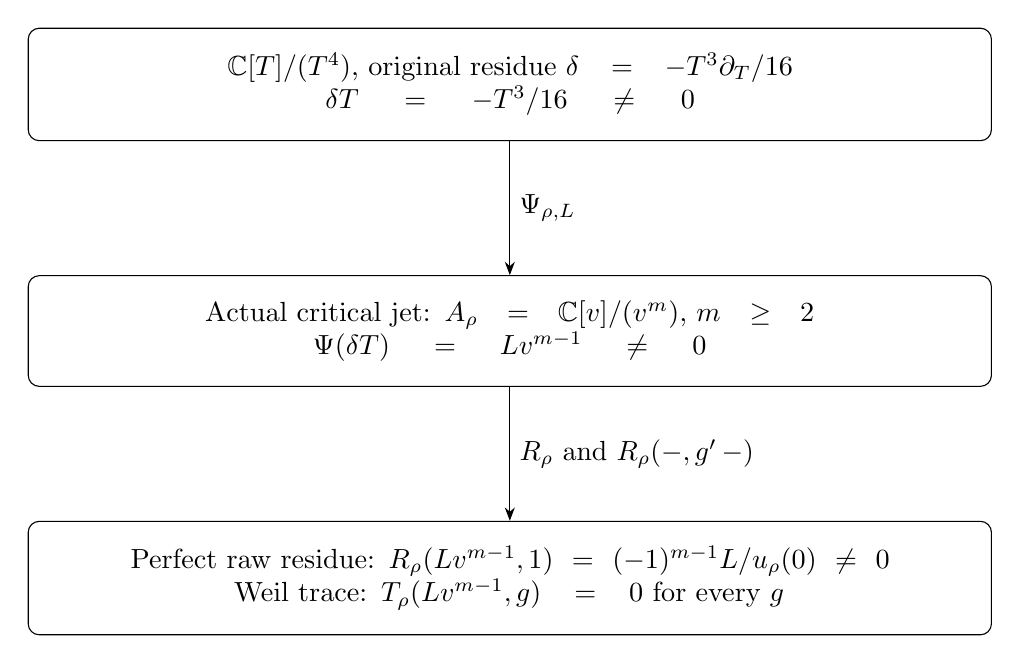
\begin{tikzpicture}[>=Stealth,node distance=1.7cm,
 box/.style={draw,rounded corners,align=center,text width=11.6cm,inner sep=9pt}]
\node[box] (source) {$\mathbb C[T]/(T^4)$, original residue
 $\delta=-T^3\partial_T/16$\\$\delta T=-T^3/16\ne0$};
\node[box,below=of source] (jet) {Actual critical jet:
 $A_\rho=\mathbb C[v]/(v^m)$, $m\ge2$\\
 $\Psi(\delta T)=Lv^{m-1}\ne0$};
\node[box,below=of jet] (pair) {Perfect raw residue:
 $R_\rho(Lv^{m-1},1)=(-1)^{m-1}L/u_\rho(0)\ne0$\\
 Weil trace: $T_\rho(Lv^{m-1},g)=0$ for every $g$};
\draw[->] (source)--node[right] {$\Psi_{\rho,L}$}(jet);
\draw[->] (jet)--node[right] {$R_\rho$ and $R_\rho(-,g'\,{-})$}(pair);
\end{tikzpicture}
\medskip
\begin{tabular}{c|c|c}
 & $a>0$ & $a=e$\\\hline
 $(a^\dagger)^2+2a-3$ & $(a-1)^2(2a+1)/a^2$ & $-3$\\[3pt]
 $(a-1)^2(2a+1)(a^\dagger)^2$ & $(a-1)^2(2a+1)/a^2$ & $e$\\[3pt]
 Difference & $e$ & $-3$
\end{tabular}
\caption{The endpoint defect has two explicitly computed receivers.
The upper diagram retains the actual eight-state residue, its full
jet image and its nonzero raw-residue value (HW61--64 and EP12--17).
For a fixed reflected zero its Weil image lies in the nilpotent radical.
The table computes the two extensions of Rodgers--Tao's exact
positive potential (EP18--21); entries retain top support and their
differences are in the top additive group. Neither calculation
identifies a negative assigned potential with a negative Weil test.}
\end{figure}



% Complete source: HOLONOMY_AND_WEIL_bibliography.tex
\begin{thebibliography}{99}
\bibitem{HW-CCcycles}
Alain Connes and Caterina Consani,
\emph{Spectral Triples and Zeta Cycles},
\href{https://arxiv.org/abs/2106.01715}{arXiv:2106.01715}.
Original author file \texttt{Spectraltriples.tex}:
lines 217--258 for the full explicit formula,
1296--1348 for periodization and scaling,
1355--1444 for Definition \texttt{zc}, Theorem
\texttt{spectralreal}, and Corollary \texttt{repetitions}.
The original archive remains intact; the private source ledger
records the exact file hash and bounded reading coverage.
\bibitem{HW-CCHH}
Alain Connes and Caterina Consani,
\emph{Hochschild homology, trace map and zeta-cycles},
\href{https://arxiv.org/abs/2207.10419}{arXiv:2207.10419}.
Original author file \texttt{Hochschild-zeta.tex}:
Proposition \texttt{laplacian}, map \texttt{evalmaprho},
Corollary \texttt{rhequiv}, lines 423--476;
final scaling-site theorem and Remark \texttt{remtauto},
lines 641--703.
\bibitem{HW-CCWeil}
Alain Connes and Caterina Consani,
\emph{Weil positivity and trace formula, the archimedean place},
\href{https://arxiv.org/abs/2006.13771}{arXiv:2006.13771},
Selecta Mathematica 27 (2021).
Original author file \texttt{weil-compo.tex}:
introduction \texttt{explicit form}, \texttt{weilnegav},
and Theorem \texttt{mainthmintro};
Appendix \texttt{apppositivity}, Proposition
\texttt{mainprop}, lines 2072--2085.
The source credits Andr\'e Weil's 1952 explicit-formula
criterion and Hiroyuki Yoshida's 1992 compact-test refinement.
No original-source reading of those historical articles is claimed.
\bibitem{HW-CCclass}
Alain Connes and Caterina Consani,
\emph{Knots, primes and class field theory},
\href{https://arxiv.org/abs/2501.06560v1}{arXiv:2501.06560v1}.
Original author file \texttt{arxiv-pisa.tex}, lines 464--691:
Definition \texttt{coverdef}, Lemma \texttt{Gacts},
Proposition \texttt{mappingtorus}, Theorem
\texttt{mappingtorus1}, Fact \texttt{artinrec}, and
Theorem \texttt{main}.
\bibitem{HW-Jensen}
Johan Ludwig William Valdemar Jensen,
\emph{Sur un nouvel et important th\'eor\`eme de la th\'eorie
des fonctions}, Acta Mathematica 22 (1899), 359--364,
\href{https://doi.org/10.1007/BF02417878}
{doi:10.1007/BF02417878}.
Historical metadata attribution; the circle argument used
here is proved in HW25--26, not inferred from an unread PDF.
\bibitem{HW-EHM}
Retained programme derivation,
\href{https://github.com/KokunoYumeto/zeta-function-research-reader/blob/adfbfe74fa49e31cb7aa068cf755fb083be37c32/workbenches/splitzero-tandem/branches/tau-zero-prime-positivity/EIGHT_STATE_HOLONOMY_DERIVATION.md}
{Eight-state holonomy, EHM27--46}.
The local family, original clock, interpolation multiplier,
and residue used here are proved again in HW61--64.
\bibitem{HW-Programme}
The retained programme source calculations are
\emph{Primitive representatives of the complete arithmetic jet packets},
PL1--28 and PL37--39, in
\texttt{PRIMITIVE\_PACKET\_LIFT.tex};
the full lattice definition and universal maps in
\texttt{split\_support\_geometry\_arithmetic\_curve\_v11.tex};
and the receiver calculations SZW6--15,
PHW2--25, HWA27--34.
All formulas used from them are rederived in this article.
The private ledger records their exact source files and reading
coverage. Their publicly available arithmetic receivers are
\href{https://github.com/KokunoYumeto/zeta-function-research-reader/blob/adfbfe74fa49e31cb7aa068cf755fb083be37c32/workbenches/splitzero-tandem/branches/tau-zero-prime-positivity/SUPPORTED_ZERO_PRIME_WEIL_DERIVATION.md}
{SZW, equations SZW6--15}
and
\href{https://github.com/KokunoYumeto/zeta-function-research-reader/blob/d5c9d198a8432e3ede468b280162a99c00e3f4f7/workbenches/splitzero-tandem/branches/tau-zero-prime-positivity/HOLONOMY_AVERAGING_WEIL_ENDPOINT_DERIVATION.md}
{HWA, equations HWA27--34}.
The present source makes no claim of publishing any previously
withdrawn exploration.
\end{thebibliography}


\end{document}
